% Created 2024-02-15 Thu 09:06
% Intended LaTeX compiler: pdflatex
\documentclass[11pt]{article}
\usepackage[utf8]{inputenc}
\usepackage[T1]{fontenc}
\usepackage{graphicx}
\usepackage{longtable}
\usepackage{wrapfig}
\usepackage{rotating}
\usepackage[normalem]{ulem}
\usepackage{amsmath}
\usepackage{amssymb}
\usepackage{capt-of}
\usepackage{hyperref}
\usepackage[margin=0.5in]{geometry}
\author{root}
\date{\today}
\title{}
\hypersetup{
 pdfauthor={root},
 pdftitle={},
 pdfkeywords={},
 pdfsubject={},
 pdfcreator={Emacs 29.1.50 (Org mode 9.6.8)}, 
 pdflang={English}}
\begin{document}


\section{My thoughts and bible references regarding theology}
\label{sec:org7a90de6}
\textbf{Acts 13:48} - And when the Gentiles heard this, they began rejoicing and glorifying the word of the Lord, and as many as were appointed to eternal life believed. (ESV)

I've been thinking about belief, faith, works, law and receiving the Holy Spirit!
Please let me know what you think if you have the time.

I'm trying to get clearer on this.
Please feel free to discuss it with me.

\textbf{Romans 10:3-4} - For, being ignorant of the righteousness that comes from God, and seeking to establish their own, they did not submit to God's righteousness. For Christ is the end of the law for righteousness to everyone who believes.

I enjoyed this video, but I still am of the opinion that keeping the law is not necessary, (but not prohibited, so long as it is pursued by faith and submitting to God's righteousness):
\begin{itemize}
\item \href{https://www.youtube.com/watch?v=CNHKqhwu6Bo}{Public Debate - Should Christians Keep The Law? - YouTube}
\end{itemize}

What I like about the didache is that it still upholds righteous living and following God's Great commandments and precepts.

\url{https://www.earlychristianwritings.com/text/didache-roberts.html}

I think it's important to live righteously out of love for God and one's neighbour, and out of faith.
That being said, I think God does justify through faith, and I believe faith works. And working may indeed be called faith if the work is done in faith.
I also think God likely saves through works because it may be their way of demonstrating faith to Jesus.

There's a false dichotomy between faith and works.

\section{Justifying faith vs justifying works is misunderstood and is a false dichotomy}
\label{sec:orga8f800a}
Because someone has bundled 'trusting
action/seeking God in action' along with
'obedience' into works when it belongs inside
faith.

\begin{itemize}
\item Obedience belongs inside faith because
\begin{itemize}
\item God commanded it and complying is not really bringing anything
to God which He hasn't told you to bring to Him.
\begin{itemize}
\item So it's just acting in faith
\item If God commands you to wait a week before going into battle, is that considered work? No, it's faith.
\end{itemize}
\item Choosing to obey God's commandments even when no-one is watching (aside from God) is having faith in God.
\begin{itemize}
\item Therefore, there is a way of abiding by God's commandments which is faith and not works.
\end{itemize}
\end{itemize}
\item Seeking God in action belongs in faith because
\begin{itemize}
\item When someone wills to seek God, they act.
\item And \textbf{Hebrews 11:6} declares that faith is implied when someone believes God exists and rewards those who seek Him.
\begin{itemize}
\item And \textbf{Hebrews 11:6} declares that God rewards those who seek Him.
\end{itemize}
\end{itemize}
\end{itemize}

'Rewards from God for seeking Him' belongs in faith, or it's not faith anymore, even in regards to justifying faith.

\textbf{Hebrews 11:6} - And without faith it is impossible to please him, for whoever would draw near to God must believe that he exists and that he rewards those who seek him.

\textbf{Hebrews 11:24-26} - By faith Moses, when he was grown up, refused to be called the son of Pharaoh's daughter, choosing rather to be mistreated with the people of God than to enjoy the fleeting pleasures of sin.  He considered the reproach of Christ greater wealth than the treasures of Egypt, for he was looking to the reward.

\subsection{The type of work that is good}
\label{sec:org2caae49}
\textbf{John 15:5} -  I am the vine; you are the branches.  Whoever abides in me and I in him, he it is that bears much fruit, for apart from me you can do nothing.  (ESV)

\subsection{The type of work that's bad}
\label{sec:org5252ca5}
'Working' for God is OK in some forms. It's a part of faith.

But what is wrong is trying to establish a righteousness of one's own apart from submitting to the righteousness of God.

\textbf{James 2:18} - But someone will say, You have faith and I have works. Show me your faith apart from your works, and I will show you my faith by my works.

\textbf{Hebrews 6:1} - Therefore let us leave the elementary doctrine of Christ and go on to maturity, not laying again a foundation of repentance from dead works and of faith toward God,

Dead works are works not done in service to God, but works dnoe in service to God, He may accept.

\textbf{Hebrews 9:14} - how much more will the blood of Christ, who through the eternal Spirit offered himself without blemish to God, purify our conscience from dead works to serve the living God.

We stop doing dead works to serve the living God, which I believe is obedience,
which is really similar to work but it's obeying. Obedience gives glory to God.

\textbf{John 13:34-35} - A new commandment I give to you, that you love one another: just as I have loved you, you also are to love one another. By this all people will know that you are my disciples, if you have love for one another. (ESV)

Obeying Jesus' commandments are not 'dead works'.

\textbf{Exodus 20:12-17} - Honor your father and your mother, that your days may be long in the land that the Lord your God is giving you.  You shall not murder.  You shall not commit adultery.  You shall not steal.  You shall not bear false witness against your neighbor.  You shall not covet your neighbor's house; you shall not covet your neighbor's wife, or his male servant, or his female servant, or his ox, or his donkey, or anything that is your neighbor's.

Jesus said:

\textbf{Mark 10:19} - You know the commandments: Do not murder, Do not commit adultery, Do not steal, Do not bear false witness, Do not defraud, Honor your father and mother. (ESV)

Obeying God by following the 10 commandments properly, in truth, is not performing 'dead works'.

\textbf{Hebrews 9:14} - how much more will the blood of Christ, who through the eternal Spirit offered himself without blemish to God, purify our conscience from dead works to serve the living God.

Service to God is obeying God through Christ's commandments. It's being a bond-servant of Christ.

\textbf{John 14:12} - Truly, truly, I say to you, whoever believes in me will also do the works that I do; and \textbf{greater works than these will he do}, because I am going to the Father.

Whoever has faith in Jesus, the works that Jesus does, that person will do.
Pisteuo = faith.

\textbf{John 14:12} - Truly (G281 amen), truly (G281 amen), I say (G3004 lego) to you, he who believes (G4100 pisteuo) in Me, the works (G2041 ergon) that I do (G4160 poieo), he will do (G4160 poieo) also (G2548 kakeinos); and greater (G3173 megas) works than these (G3778 houtos) he will do (G4160 poieo); because (G3754 hoti) I go (G4198 poreuomai) to the Father (G3962 pater).

\begin{verbatim}
1  :  4100  pisteuo  pist-yoo'-o
2  
3   from 4102; to have faith (in, upon, or with respect to, a person or
4   thing), i.e. credit; by implication, to entrust (especially one's
5   spiritual well-being to Christ):--believe(-r), commit (to trust), put
6   in trust with.
7   see GREEK for 4102
\end{verbatim}

If someone trusts their Lord then they do what their Lord does and has commanded.

Faith has an amount.
I think even saving faith requires an amount.
Shear fear of God or love for Him is work which comes out of belief.
But faith works, even saving faith works.
Faith without work doesn't exist I think - but the work can come from Jesus, I think.
For example, with Lazarus - Jesus performed the work so the people watching could believe and have faith.

\textbf{John 11:42} - I knew that you always hear me, but I said this on account of the people standing around, that they may believe that you sent me.

And Jesus is able to save a person out of Jesus' own will, as he resurrected Lazarus.

\textbf{John 11:43} - When He had said these things, He cried out with a loud voice, “Lazarus, come forth.”

But faith is like Peter stepping out on the water. Faith works. But I think sometimes to create faith someone just has to actually believe Jesus because Jesus performs the miracle / the work. The account of Jesus itself when it's read, and Jesus' words, are enough to inspire faith. Jesus calls persistent endurance a work. Therefore, faith comes by hearing the word of Christ.

\textbf{Ephesians 2:8-9} - For by grace you have been saved through faith. And this is not your own doing; it is the gift of God, not a result of works, so that no one may boast.

I think \textbf{Ephesians 2:8-9} when it says 'through faith' doesn't actually exclude obedience (obeying Jesus), because I think obedience is intrinsic to faith.

When it says "not a result of works", I believe that something more like, even if works were tied into the faith, it's by grace. If a person's saving faith included works then that is fine.

I believe in all of theses:
\begin{itemize}
\item \texttt{sola fida} (by faith alone) AMEN!!.
\begin{itemize}
\item The justifying faith may include 'acts of faith', which is just visible faith.
\item Works done outside of faith \textbf{do not} qualify for justification.
\end{itemize}
\item \texttt{sola gratia} (by grace alone) AMEN!!
\item \texttt{sola scriptura} (by Scripture alone) AMEN!!
\item \texttt{Solus Christus} AMEN!!
\item \texttt{Soli Deo gloria} (glory to God alone) AMEN!! But the glory God gives us glorifies God.
\begin{itemize}
\item When it comes to forgiving offenses of others, my understanding is that it is about forgiving others' offenses against 'you', thereby ultimately still going through Christ for forgiveness, since
\item \textbf{John 20:22-23} - And when he had said this, he breathed on them and said to them, Receive the Holy Spirit. (ESV)
\item \textbf{Proverbs 19:11} - Good sense makes one slow to anger, and it is his glory to overlook an offense. (ESV)
\item \textbf{Matthew 6:12} - and forgive us our debts, as we also have forgiven our debtors.
\item \textbf{Matthew 18:35} - So also my heavenly Father will do to every one of you, if you do not forgive your brother from your heart.
\item \textbf{Mark 11:25} - And whenever you stand praying, forgive, if you have anything against anyone, so that your Father also who is in heaven may forgive you your trespasses.
\item \textbf{Ephesians 4:32} - Be kind to one another, tender-hearted, forgiving each other, just as God in Christ also has forgiven you.
\item \textbf{Matthew 10:8} -  Heal the sick, raise the dead, cleanse lepers, cast out demons.  You received without paying; give without pay. (ESV)
\end{itemize}
\end{itemize}

Hearing God's word and believing it, and even acting on it, like Peter stepping out on the water, or like the woman at the well going in to town to tell people about Jesus, or turning from sinful things. And there is an amount of faith, and true belief is all that's required to be saved, but Faith is so tightly linked to Obedience like Faith is linked to Hope. True belief is enough because it accepts what Jesus says, as a child believes. But I don't think this discounts faith that increases through obedience.

Peter demonstrated obedience. A changed heart is essential to be saved, I think.

Hebrews describes faith as hope with belief in reward from seeking God.

\textbf{Hebrews 11:1} - Now faith is the assurance of things hoped for, the conviction of things not seen.

\textbf{Hebrews 11:6} - And without faith it is impossible to please him, for whoever would draw near to God must believe that he exists and that he rewards those who seek him.

The whole chapter of Hebrews 11 also describes many 'acts' of faith. Belief and action are like a vector.

\documentclass{article}
\usepackage{tikz}
\usepackage{amsmath}
\begin{document}
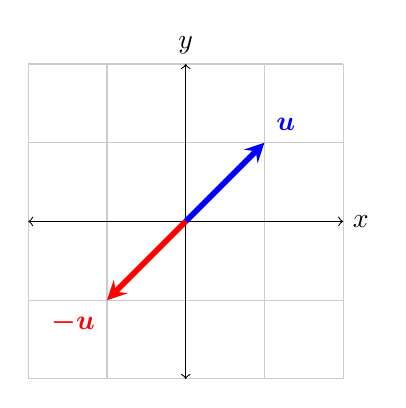
\begin{tikzpicture}
  \draw[thin,gray!40] (-2,-2) grid (2,2);
  \draw[<->] (-2,0)--(2,0) node[right]{$x$};
  \draw[<->] (0,-2)--(0,2) node[above]{$y$};
  \draw[line width=2pt,blue,-stealth](0,0)--(1,1) node[anchor=south west]{$\boldsymbol{u}$};
  \draw[line width=2pt,red,-stealth](0,0)--(-1,-1) node[anchor=north east]{$\boldsymbol{-u}$};
\end{tikzpicture}
\end{document}

\begin{verbatim}
 1  Faith = Hope-from/in-God * Work/Love
 2  
 3  Hope-from/in-God = Belief(believing God) * Truth(God's word is truth)
 4  
 5  Work/Love = Obedience * Faithfulness * Fear-of-God * Response-of-love-to-Jesus * Patient-Endurance(time)
 6  
 7  Obedience = Submitting to the Righteousnes of God + Turning from sin, loving, showing mercy, etc.
 8  
 9  Fear-of-God = e.g. The poor in spirit recognise their need of God's mercy and tremble at His Word: "beat his breast, saying, God, be merciful to me, a sinner!"
10  
11  Response-of-love-to-Jesus = e.g. praise, thankfulness, obeying His commandments
\end{verbatim}

Faith has 'substance' and may be described as a vector:
\begin{itemize}
\item Hope-from/in-God is the direction.
\item Work/Love is the magnitude.
\end{itemize}

But it's God that tests the faith, and God that justifies. That's why I don't like making an assertion on the exact way that God justifies, because God is the justifier.

\textbf{Romans 8:33} -  Who shall bring any charge against God's elect?  It is God who justifies.  (ESV)

The outcome is eternal life.

\textbf{Romans 6:22-23} - But now that you have been set free from sin and have become slaves to God, the fruit you reap leads to holiness, and the outcome is eternal life. For the wages of sin is death, but the gift of God is eternal life in Christ Jesus our Lord. (BSB)

A person must \textbf{do} the will of Father God; They must be obedient.
Faith and obedience are inseparable.

\textbf{Matthew 7:21-23} -  Not everyone who says to me, Lord, Lord, will enter the kingdom of heaven, but the one who does the will of my Father who is in heaven.  On that day many will say to me, Lord, Lord, did we not prophesy in your name, and cast out demons in your name, and do many mighty works in your name?  And then will I declare to them, I never knew you; depart from me, you workers of lawlessness. (ESV)

The works have to be the will of Father God.

\subsection{Justifying faith should result in going from disobedient to obedient}
\label{sec:org456dd95}

\textbf{II Corinthians 10:5-6} - We destroy arguments and every lofty opinion raised against the knowledge of God, and take every thought captive to obey Christ, being ready to punish every disobedience, when your obedience is complete.

\textbf{Ephesians 2:2} - in which you once walked, following the course of this world, following the prince of the power of the air, the spirit that is now at work in the sons of disobedience—

\textbf{Ephesians 5:6} - Let no one deceive you with empty words, for because of these things the wrath of God comes upon the sons of disobedience.

Now obeying God is more than just believing, it's obeying (which is proportional to the magnitude of the faith).

Understand that the ones who remained in the boat and did not step out onto the water did not have enough faith to walk on water.

\textbf{Matthew 14:27-32} - But immediately Jesus spoke to them, saying, Take heart; it is I. Do not be afraid.  And Peter answered him, Lord, if it is you, \textbf{command} me to come to you on the water.  He said, Come. So Peter \textbf{got out of the boat and walked on the water and came to Jesus}.  But when he saw the wind, he was afraid, and beginning to sink he cried out, Lord, save me.  Jesus immediately reached out his hand and took hold of him, saying to him, O you of little faith, why did you doubt?  And when they got into the boat, the wind ceased.

Fear made them disobedient. They had only a small amount of faith.

\textbf{Hebrews 2:2} - For since the message declared by angels proved to be reliable and every transgression or disobedience received a just retribution,

\textbf{Hebrews 9:14} - how much more will the blood of Christ, who through the eternal Spirit offered himself without blemish to God, purify our conscience from dead works to serve the living God.

\subsection{Obedience is essential to justifying faith}
\label{sec:orgd44a697}
\textbf{Hebrews 4:6} - Since therefore it remains for some to enter it, and those who formerly received the good news failed to enter because of disobedience,

\textbf{Hebrews 4:11} - Let us therefore strive to enter that rest, so that no one may fall by the same sort of disobedience.

\textbf{I John 2:17} - And the world is passing away along with its desires, but \textbf{whoever does the will of God abides forever}.

\subsection{Jesus' odedience resulted in turning others to obedience}
\label{sec:orga05cc0c}
\textbf{Romans 5:19} - For as by the one man's disobedience the many were made sinners, so by the one man's obedience the many \textbf{will be made} righteous.

A process:
\begin{itemize}
\item 'Will be made' => Turning people to obedience.
\end{itemize}

\subsection{It is the mercy of God that we are turned from obedience to obedience}
\label{sec:org7db4400}
I think that is the correct way to see the following Scripture:

\textbf{Romans 11:29-33}: For the gifts and the calling of God are irrevocable.  Just as you were at one time disobedient to God but now have received mercy because of their disobedience, so they too have now been disobedient in order that by the mercy shown to you they also may now receive mercy.  For God has consigned all to disobedience, that he may have mercy on all.  Oh, the depth of the riches and wisdom and knowledge of God! How unsearchable are his judgments and how inscrutable his ways!

\subsection{What we hear and how we hear}
\label{sec:org6f3e36e}
\textbf{Mark 4:24} - And he said to them, Pay attention to what you hear: with the measure you use, it will be measured to you, and still more will be added to you.

\textbf{Luke 8:18} - So take care how you listen; for whoever has, to him more shall be given; and whoever does not have, even what he thinks he has shall be taken away from him.”

If you do not take care of \texttt{how} you hear and \texttt{what} you hear, then \ldots{}

\textbf{Isaiah 6:10} - “Render the hearts of this people insensitive, Their ears dull, And their eyes dim, Otherwise they might see with their eyes, Hear with their ears, Understand with their hearts, And return and be healed.”

I think it's important to take in all the words which Jesus spoke which are available to us, and to come to a faith which is able to reconcile faith with works, and law and obedience, and the gospel Jesus taught before and after the resurrection, and reconcile the teachings of the epistles from Peter, Paul and John, and Epistle to the Hebrews.

\textbf{Matthew 13:15} - For the heart of this people has become dull, With their ears they scarcely hear, And they have closed their eyes, Otherwise they would see with their eyes, Hear with their ears, And understand with their heart and \textbf{return}, And I would heal them.’

The word return specifies 'action'.

\textbf{John 12:40} - “He has blinded their eyes and He hardened their heart, so that they would not see with their eyes and perceive with their heart, and be converted and I heal them.”

\textbf{Acts 28:27} - For the heart of this people has become dull, And with their ears they scarcely hear, And they have closed their eyes; Otherwise they might see with their eyes, And hear with their ears, And understand with their heart and \textbf{return}, And I would heal them.”’

\subsubsection{Garden of Eden}
\label{sec:org102f9dd}
\begin{itemize}
\item Eve listened to another voice
\end{itemize}

If you listen to someone with a deceptive, beguiling spirit, then the same measure of that would come into you.

And that would would probably affect the truthfulness of your dreams if you have a prophetic gift.

\section{laws}
\label{sec:orge4c8394}
\begin{itemize}
\item Great commandments
\begin{itemize}
\item to love the Lord your God with all your heart, soul, mind and strength and your neighbour as yourself
\end{itemize}
\item 10 Commandments
\item the 613 Mosaic laws
\item the law of Christ
\end{itemize}

\section{Commandments and faith}
\label{sec:org17a52cb}
\textbf{Revelation of John 14:12} - Here is a call for the endurance of the saints, those who keep the commandments of God and their faith in Jesus.

I read this as 'A saint is someone who has faith in Jesus AND keeps the commandments (pursuing by faith, not works)'.
I read this as the Great commandments, 10 Commandments and faith in Jesus Christ, and potentially various other commandments from the Mosaic law if you now about them, or whatever subset a person practices.
But the law should be pursued by faith and not by works.

\textbf{John 15:10} - If you keep my commandments, you will abide in my love, just as I have kept my Father's commandments and abide in his love.

\textbf{Romans 9:30-32} - What shall we say, then? That Gentiles who did not pursue righteousness have attained it, that is, a righteousness that is by faith; but that Israel who pursued a law that would lead to righteousness did not succeed in reaching that law. Why? Because they did not pursue it by faith, but as if it were based on works. They have stumbled over the stumbling stone, (ESV)

Jesus' commandments don't contradict the rest of the commandments.

Also God's commandments (especially the 10 Commandments; loving God and your neighbour) are still binding on us - written on our heart when we get born-again and after being born-again we follow them in Spirit.

Jesus fulfilled the law => We have the Spirit of Christ => We are led by the Spirit and naturally want to follow the law in faith but the world opposes us because when a person actually follows the commandments, they do not lie, do not commit adultery, do not commit idolatry, etc. and that means a person can be taken advantage of.
But we don't pursue the law by works. We are freed from being under the law, and the curse of the law to serve and obey God in truth, being under God's grace.

\textbf{Romans 7:6} -  But now we are released from the law, having died to that which held us captive, so that we serve not under the old written code but in the new life of the Spirit.  (ESV)

This is still following the law but in faith and in Spirit, not being under the law.

\textbf{Deuteronomy 4:13} - And he declared to you his covenant, which he commanded you to perform, that is, the Ten Commandments, and he wrote them on two tablets of stone.

\textbf{Romans 10:5} - For Moses writes about the righteousness that is based on the law, that the person who does the commandments shall live by them.

\textbf{Romans 13:9} - The commandments, You shall not commit adultery, You shall not murder, You shall not steal, You shall not covet, and any other commandment, are summed up in this word: You shall love your neighbor as yourself.

There's no contradiction.

However, we must submit to God's righteousness through faith in Jesus Christ.

The Mosaic law is not abolished but Jesus fulfilled it like a prophesy.

The righteousness we have through faith in Jesus Christ is needed whether someone keeps the Mosaic law or not.
Not that I keep the Mosaic law in its entirety, nor are circumcised. But I try to keep the Great commandments
and the 10 Commandments out of faith (and a relationship with God) and follow parts of the Mosaic law,
but I have faith in Jesus Christ for the righteousness that comes through faith because I need that because my own
righteousness will never be enough without faith in Jesus for God's righteousness imputed to me.

Thank You God.

\textbf{Ephesians 2:8} -  For by grace you have been saved through faith.  And this is not your own doing; it is the gift of God,  (ESV)

AMEN!!

\textbf{Galatians 2:17} -- But if, in our endeavor to be justified in Christ, we too were found to be sinners, is Christ then a servant of sin? Certainly not! (ESV)

AMEN!!

\textbf{Romans 10:3-4} - For, being ignorant of the righteousness that comes from God, and seeking to establish their own, they did not submit to God's righteousness. For Christ is the end of the law for righteousness to everyone who believes.

This is why we are not \textbf{under} the law because we have the righteousness that comes through faith in Christ.

But we are under the law of faith in Christ.
And we are supposed to keep the commandments by pursuing them in faith.

\section{Jesus fulfilled the law}
\label{sec:org4198e1d}
\begin{itemize}
\item Who gave Moses the law and the instructions to build the tabernacle? God did.
\begin{itemize}
\item The blueprints came from God.
\end{itemize}
\item The Law, the Psalms and the Prophets all point to Jesus.
\item Moses wrote about Jesus.
\item Jesus fulfilled the Law and the prophesies.
\end{itemize}

We still follow the law but by faith and not by works.

We keep accountability with God, and in truth over following the law - God knows when we lie, cheat, commit adultery, idolise etc.
We follow the law in truth.
Jesus fulfilled the law. Jesus' blood is the atonement for sin.
So we go to Jesus for forgiveness instead of perform the ceremonial law to try to make atonement for sin.

This looks like an interesting resource about that - \url{http://www.abideinchrist.com/messages/tabernacletype.html}

\subsection{Justified by faith alone}
\label{sec:orgb8a6fd7}
I think someone who trusts in God to save them through saving faith in Jesus Christ, is saved, or is in the process of being saved.

God is the judge of what saving faith looks like, and how long the process of 'being saved' takes.

The Revelation of John shows that Jesus looks at people's works.

Faith without working through love doesn't count for anything.

\subsubsection{Saving faith - believing and observing Jesus' work}
\label{sec:orge27424a}
Faith may come from simply observing Jesus work, or through work from
disciples of Jesus.

\textbf{John 11:14-15} Then Jesus told them plainly, Lazarus has died, and for your sake I am glad that I was not there, so that you may believe. But let us go to him.

It's for their sake, so that they would be able to believe (have faith).

\textbf{John 11:15} - and I am (G5463 chairo) glad (G5463 chairo) for your sakes (G1223 dia) that I was not there (G1563 ekei), so (G2443 hina) that you may believe (G4100 pisteuo); but let us go (G71 ago) to him.”

\begin{verbatim}
1  :  4100  pisteuo  pist-yoo'-o  
2  
3   from 4102; to have faith (in, upon, or with respect to, a person or
4   thing), i.e. credit; by implication, to entrust (especially one's
5   spiritual well-being to Christ):--believe(-r), commit (to trust), put
6   in trust with.
7   see GREEK for 4102
\end{verbatim}

\textbf{John 11:23-27} - Jesus said to her, Your brother will rise again.  Martha said to him, I know that he will rise again in the resurrection on the last day.  Jesus said to her, I am the resurrection and the life. Whoever believes in me, though he die, yet shall he live, and everyone who lives and believes in me shall never die. Do you believe this?  She said to him, Yes, Lord; I believe that you are the Christ, the Son of God, who is coming into the world.

The person has to \textbf{really} believe - to have actual faith.
Even Martha's faith here was put on display when she confessed,
"Yes, Lord; I believe that you are the Christ, the Son of God, who is coming into the world."
It shows she has faith.

\subsubsection{Saving faith - by the grace of God alone - no works of faith}
\label{sec:org5fb532f}
Yes, I think it's possible, but I wouldn't guarantee it.

\textbf{John 11:25} - Jesus said to her, I am the resurrection and the life. Whoever believes in me, though he die, yet shall he live,

AMEN!!

\textbf{True} belief is enough to be spared from death.
However, I still think that inheriting the Kingdom is different.

\subsubsection{Saving faith - a life of faith}
\label{sec:orgfd3f0e3}
I believe there's a difference between being spared from condemnation and receiving eternal life.

\textbf{Romans 6:22} - But now that you have been set free from sin and have become slaves of God, the fruit you get leads to sanctification and its end, eternal life.

Eternal life is totally different - it's becoming a part of the Truth - it's union with Christ and with God.

\textbf{Matthew 19:29} -  And everyone who has left houses or brothers or sisters or father or mother or children or lands, for my name's sake, will receive a hundredfold and will inherit eternal life.  (ESV)

\subsubsection{Saving faith / Works of faith}
\label{sec:org0352b35}
Jesus said that patient endurance is a work.

Likewise, love for Jesus also qualifies as a work.

\textbf{Mark 11:23} - Truly, I say to you, whoever \textbf{says to this mountain, Be taken up and thrown into the sea}, and \textbf{does not doubt in his heart}, but believes that what he says \textbf{will come to pass}, it will be done for him.

Saving faith with work (yes, obedience is intrinsic to faith, like belief):

\textbf{Matthew 14:28-31} - And Peter answered him, Lord, if it is you, command me to come to you on the water.  He said, Come. So Peter got out of the boat and walked on the water and came to Jesus.  But when he saw the wind, he was afraid, and beginning to sink he cried out, Lord, save me.  Jesus immediately reached out his hand and took hold of him, saying to him, O you of little faith, why did you doubt?

Obeying Jesus' commandments - believing Jesus and acting on Jesus' commandments \textbf{is} faith.

\subsubsection{Faith with works}
\label{sec:org20d758f}
James isn't talking about work of the law, he's talking about the works of faith.

\textbf{James 2:13-17} - For judgment is without mercy to one who has shown no mercy. Mercy triumphs over judgment. What good is it, my brothers, if someone says he has faith but does not have works? Can that faith save him? If a brother or sister is poorly clothed and lacking in daily food, and one of you says to them, Go in peace, be warmed and filled, without giving them the things needed for the body, what good is that? So also faith by itself, if it does not have works, is dead.

Faith without work is dead; it's useless.

That person is completely at the mercy of Jesus and of the saints, I think.

Sometimes a person's work is all burned up but they are \textbf{still saved}.

\textbf{1 Corinthians 3:15} -  If anyone's work is burned up, he will suffer loss, though he himself will be saved, but only as through fire. (ESV)

I think then someone must be prepared to accept salvation through grace alone because they need it.

\subsection{Working faith / faith with substance}
\label{sec:org7b399e7}

Faith is a relationship with God. God has promised inheriting the Kingdom, inheriting eternal life to those who obey Him. But God is sovereign to save.

My equations:

\begin{verbatim}
 1  Faith = Hope-from/in-God * Work/Love
 2  
 3  Hope-from/in-God = Belief(believing God) * Truth(God's word is truth)
 4  
 5  Work/Love = Obedience * Faithfulness * Fear-of-God * Response-of-love-to-Jesus * Patient-Endurance(time)
 6  
 7  Obedience = Submitting to the Righteousnes of God + Turning from sin, loving, showing mercy, etc.
 8  
 9  Fear-of-God = e.g. The poor in spirit recognise their need of God's mercy and tremble at His Word: "beat his breast, saying, God, be merciful to me, a sinner!"
10  
11  Response-of-love-to-Jesus = e.g. praise, thankfulness, obeying His commandments
\end{verbatim}

But salvation is a gift and God is sovereign to save.
That's why it's grace.
Saved by grace through faith.

I think a person needs \textbf{some} faith to be saved.

\textbf{Ephesians 2:8} -  For by grace you have been saved through faith.  And this is not your own doing; it is the gift of God,  (ESV)

Mercy is available:

\textbf{Luke 18:13} -  But the tax collector, standing far off, would not even lift up his eyes to heaven, but beat his breast, saying, God, be merciful to me, a sinner!  (ESV)

Those who fear God inherit the Kingdom.

\textbf{Matthew 5:3} - Blessed are the poor in spirit, for theirs is the kingdom of heaven.

\begin{center}
\begin{tabular}{ll}
Condition & Promise\\[0pt]
\hline
Some will be inherit the kingdom of Heaven & Those who are poor in spirit\\[0pt]
\end{tabular}
\end{center}

\textbf{Isaiah 66:2} -  All these things my hand has made, and so all these things came to be, declares the LORD.  But this is the one to whom I will look: he who is humble and contrite in spirit and trembles at my word.  (ESV)

We need faithfulness and not faithlessness and disbelief to inherit the promises:

\textbf{Hebrews 12:16-17} - that no one is sexually immoral or unholy like Esau, who sold his birthright for a single meal. For you know that afterward, when he desired to inherit the blessing, he was rejected, for he found no chance to repent, though he sought it with tears.

\textbf{Revelation of John 2:2} - I know your works, your toil and your patient endurance, and how you cannot bear with those who are evil, but have tested those who call themselves apostles and are not, and found them to be false.

Here it says that unless the church \textbf{does the work} which it had started out doing, their lampstand will be removed from its place.

\textbf{Revelation of John 2:5} - Remember therefore from where you have fallen; repent, and do the works you did at first. If not, I will come to you and remove your lampstand from its place, unless you repent.

A response of love for Jesus \textbf{is} justifying work.

\textbf{Luke 7:47-50} -  Therefore I tell you, her sins, which are many, are forgiven-for she loved much.  But he who is forgiven little, loves little.  And he said to her, Your sins are forgiven.  Then those who were at table with him began to say among themselves, Who is this, who even forgives sins?  And he said to the woman, Your faith has saved you; go in peace.  (ESV)

\textbf{James 2:22-25} - You see that faith was active along with his works, and faith was completed by his works; and the Scripture was fulfilled that says, Abraham believed God, and it was counted to him as righteousness-and he was called a friend of God.  You see that a person is justified by works and not by faith alone.  And in the same way was not also Rahab the prostitute justified by works when she received the messengers and sent them out by another way?

ONLY \textbf{working faith} counts for anything. Even Paul agrees. However, it says 'in Christ Jesus', and I believe that those who trust in Jesus without work still abide, but by the skin of their teeth.

\textbf{Galatians 5:6} - For in Christ Jesus neither circumcision nor uncircumcision counts for anything, but \textbf{only faith working through love}. (ESV)

Loving God is obeying His commandments.

\textbf{I John 5:2-3} - By this we know that we love the children of God, when we love God and obey his commandments. For this is the love of God, that we keep his commandments. And his commandments are not burdensome.

\subsection{Entering into life / the Kingdom of Heaven}
\label{sec:org528c972}
\begin{itemize}
\item Keeping the commandments (10 commandments, from the heart, and in reality, accountable to God / the 2 Great commandments) is important for entering into the Kingdom of Heaven, entering into life.
\item Also, lay up treasure in Heaven.
\item Also, follow Jesus.
\end{itemize}

\subsubsection{Follow the commandments (get out of falsehood; stop sinning) and put your heart in Heaven}
\label{sec:orge78295d}
\textbf{Matthew 6:19-21} - Do not lay up for yourselves treasures on earth, where moth and rust destroy and where thieves break in and steal, but lay up for yourselves treasures in heaven, where neither moth nor rust destroys and where thieves do not break in and steal.  For where your treasure is, there your heart will be also.

\emph{\textbf{Loving God is obedience to God.}}

\textbf{I John 5:2-3} - By this we know that we love the children of God, when we love God and obey his commandments. For this is the love of God, that we keep his commandments. And his commandments are not burdensome.

AMEN!!

Obey God, put your heart in Heaven, follow Jesus.

\textbf{Matthew 19:16-26} - And behold, a man came up to him, saying, Teacher, what good deed must I do to have eternal life?  And he said to him, Why do you ask me about what is good? There is only one who is good. If you would enter life, keep the commandments.  He said to him, Which ones? And Jesus said, You shall not murder, You shall not commit adultery, You shall not steal, You shall not bear false witness, Honor your father and mother, and, You shall love your neighbor as yourself.  The young man said to him, All these I have kept. What do I still lack?  Jesus said to him, If you would be perfect, go, sell what you possess and give to the poor, and you will have treasure in heaven; and come, follow me.  When the young man heard this he went away sorrowful, for he had great possessions.  And Jesus said to his disciples, Truly, I say to you, only with difficulty will a rich person enter the kingdom of heaven.  Again I tell you, it is easier for a camel to go through the eye of a needle than for a rich person to enter the kingdom of God.  When the disciples heard this, they were greatly astonished, saying, Who then can be saved?  But Jesus looked at them and said, With man this is impossible, but with God all things are possible.

AMEN!!

\subsubsection{Then arriving at eternal life - follow Jesus}
\label{sec:org134f0d6}
\textbf{Matthew 19:17-21} - And he said to him, Why do you ask me about what is good? There is only one who is good. If you would enter life, keep the commandments.  He said to him, Which ones? And Jesus said, You shall not murder, You shall not commit adultery, You shall not steal, You shall not bear false witness, Honor your father and mother, and, You shall love your neighbor as yourself.  The young man said to him, All these I have kept. What do I still lack?  Jesus said to him, If you would be perfect, go, sell what you possess and give to the poor, and you will have treasure in heaven; and come, follow me.

\subsection{We are certainly supposed to keep the commandments - we're supposed to love God and our neighbour in truth}
\label{sec:org9f81f26}
\subsubsection{Keeping the commandments is how to love.}
\label{sec:orgf4e520b}

\textbf{Romans 13:9} - The commandments, You shall not commit adultery, You shall not murder, You shall not steal, You shall not covet, and any other commandment, are summed up in this word: You shall love your neighbor as yourself.

AMEN!!

\textbf{Galatians 5:14} - For the whole law is fulfilled in one word: You shall love your neighbor as yourself.

AMEN!!

\textbf{James 2:8-13} - If you really fulfill the royal law according to the Scripture, You shall love your neighbor as yourself, you are doing well.  But if you show partiality, you are committing sin and are convicted by the law as transgressors.  For whoever keeps the whole law but fails in one point has become accountable for all of it.  For he who said, Do not commit adultery, also said, Do not murder. If you do not commit adultery but do murder, you have become a transgressor of the law.  So speak and so act as those who are to be judged under the law of liberty.  For judgment is without mercy to one who has shown no mercy. Mercy triumphs over judgment.

AMEN!!

\textbf{Romans 2:13} - For it is not the hearers of the law who are righteous before God, but the doers of the law who will be justified. (ESV)

Yup - and in truth. I think the commandments often need to be looked at to see what loving looks like.

\textbf{Romans 3:31} - Do we then overthrow the law by this faith? By no means! On the contrary, we uphold the law. (ESV)

AMEN!!

\subsubsection{It matters that we are loving, going into eternity}
\label{sec:orge2ce4cc}
\textbf{Matthew 5:30} -  And if your right hand causes you to sin, cut it off and throw it away.  For it is better that you lose one of your members than that your whole body go into hell.  (ESV)

\textbf{Matthew 18:3} - and said, Truly, I say to you, unless you turn and become like children, you will never enter the kingdom of heaven.

\textbf{Matthew 18:9} - And if your eye causes you to sin, tear it out and throw it away. It is better for you to enter life with one eye than with two eyes to be thrown into the hell of fire.

\subsubsection{We must submit to the righteousness from God through faith in Jesus}
\label{sec:orgafe0aac}
\textbf{Romans 10:3-5} - For, being ignorant of the righteousness that comes from God, and seeking to establish their own, they did not submit to God's righteousness.  For Christ is the end of the law for righteousness to everyone who believes.  For Moses writes about the righteousness that is based on the law, that the person who does the commandments shall live by them.

Following the law is how to love. It's always important.

Following Jesus is having faith in Him.

Submitting to the righteousness that comes through having faith in Jesus is believing and obeying the Gospel.

\subsubsection{The honour is for those who believe}
\label{sec:org7683196}
Have faith in Jesus.
Now even someone who keeps the commandments may not obey the gospel.
The honour goes to those who obey the gospel, and believe the gospel.

\textbf{I Peter 2:6-25} - For it stands in Scripture: Behold, I am laying in Zion a stone, a cornerstone chosen and precious, and whoever believes in him will not be put to shame.  So the honor is for you who believe, but for those who do not believe, The stone that the builders rejected has become the cornerstone, and A stone of stumbling, and a rock of offense. They stumble because they disobey the word, as they were destined to do.  But you are a chosen race, a royal priesthood, a holy nation, a people for his own possession, that you may proclaim the excellencies of him who called you out of darkness into his marvelous light.  Once you were not a people, but now you are God's people; once you had not received mercy, but now you have received mercy.  Beloved, I urge you as sojourners and exiles to abstain from the passions of the flesh, which wage war against your soul.  Keep your conduct among the Gentiles honorable, so that when they speak against you as evildoers, they may see your good deeds and glorify God on the day of visitation.  Be subject for the Lord's sake to every human institution, whether it be to the emperor as supreme, or to governors as sent by him to punish those who do evil and to praise those who do good.  For this is the will of God, that by doing good you should put to silence the ignorance of foolish people.  Live as people who are free, not using your freedom as a cover-up for evil, but living as servants of God.  Honor everyone. Love the brotherhood. Fear God. Honor the emperor.  Servants, be subject to your masters with all respect, not only to the good and gentle but also to the unjust.  For this is a gracious thing, when, mindful of God, one endures sorrows while suffering unjustly.  For what credit is it if, when you sin and are beaten for it, you endure? But if when you do good and suffer for it you endure, this is a gracious thing in the sight of God.  For to this you have been called, because Christ also suffered for you, leaving you an example, so that you might follow in his steps.  He committed no sin, neither was deceit found in his mouth.  When he was reviled, he did not revile in return; when he suffered, he did not threaten, but continued entrusting himself to him who judges justly.  He himself bore our sins in his body on the tree, that we might die to sin and live to righteousness. By his wounds you have been healed.  For you were straying like sheep, but have now returned to the Shepherd and Overseer of your souls.

\section{Faith}
\label{sec:org4bfdabe}
One must have faith to receive the gift of salvation.

\textbf{Mark 11:22} - And Jesus answered them, Have faith in God.

The basic Faith equation is Believing-God * Obedience/Action/Work.

\textbf{Mark 11:23} - Truly, I say to you, whoever \textbf{says to this mountain, Be taken up and thrown into the sea}, and \textbf{does not doubt in his heart}, but believes that what he says \textbf{will come to pass}, it will be done for him.

\textbf{Mark 11:24} - Therefore I tell you, whatever you ask in prayer, believe that you have received it, and it will be yours.

Here, asking God in prayer is the work.

\section{Receiving the Holy Spirit}
\label{sec:orgeb355bb}
\subsection{The Holy Spirit cleanses the heart by faith}
\label{sec:org677b8ea}
\textbf{Acts 15:7} - And after there had been much debate, Peter stood up and said to them, Brothers, you know that in the early days God made a choice among you, that by my mouth the Gentiles should hear the word of the gospel and believe.

\textbf{Acts 15:8-9} - And God, who knows the heart, bore witness to them, by giving them the Holy Spirit just as he did to us, and he made no distinction between us and them, having cleansed their hearts by faith.

For example, out of faith in trying to follow the 10 Commandments / 2 Great Commandments, the heart is cleaned by the Holy Spirit.

Faith involves obedience. It's repentance from sin to the aligning of the heart to God's commandments.

\subsection{The faith itself may be a gift, but certainly is cooperative}
\label{sec:org1500aea}
God and Abram (Abraham) had a real relationship first.

God spoke to Abram first, and then Abram \textbf{obeyed}.
Abraham was faithful.
God noticed Abram's faithfulness, and told Abram he would be rewarded.
God gave Abram a promise.
Abram believed God.

But God made the first move.
The first move from Abraham's perspective was obedience, followed by belief.

The Lord God spoke first - this itself is a gift. We have the Bible and the testimony of others as a gift from God.
We must then believe what is said in the Holy Scriptures and trust it and obey it (put into practice).

The Holy Spirit goes to those who obey God, and causes the person to walk in God's precepts - stopping lying, stealing, coveting, idolizing, cheating, etc.

\textbf{Acts 5:32} - And we are witnesses to these things, and so is the Holy Spirit, whom God has given to those who obey him. (ESV)

Faith involves:
\begin{itemize}
\item Obedience
\item Loyalty (faithfulness to God)
\item God rewarded Abram with a promise
\item Abram believed God
\item God counted Abram's belief as righteousness
\end{itemize}

\textbf{Genesis 12:1} - Now the Lord said to Abram, Go from your country and your kindred and your father's house to the land that I will show you.

Abraham \textbf{obeyed} God.

\textbf{Genesis 12:4} - So Abram went, as the Lord had told him, and Lot went with him. Abram was seventy-five years old when he departed from Haran.

God promised him something, and gave Abram an instruction.

\textbf{Genesis 13:14} - The Lord said to Abram, after Lot had separated from him, Lift up your eyes and look from the place where you are, northward and southward and eastward and westward, for all the land that you see I will give to you and to your offspring forever.  I will make your offspring as the dust of the earth, so that if one can count the dust of the earth, your offspring also can be counted. Arise, walk through the length and the breadth of the land, for I will give it to you.

Abram obeyed.

\textbf{Genesis 13:18} - So Abram moved his tent and came and settled by the oaks of Mamre, which are at Hebron, and there he built an altar to the Lord.

OBEDIENCE!

\textbf{Hebrews 5:9-10} - And being made perfect, he became the source of eternal salvation to all who \textbf{obey} him, being designated by God a high priest after the order of Melchizedek.

Abram interacted with Melchizedek, priest of God Most High, blessed by God Most High. Abram was faithful to God even when God wasn't speaking directly to Him. God can see everything though.

\textbf{Genesis 14:18-20} - And Melchizedek king of Salem brought out bread and wine. (He was priest of God Most High. ) And he blessed him and said, Blessed be Abram by God Most High, Possessor of heaven and earth; and blessed be God Most High, who has delivered your enemies into your hand! And Abram gave him a tenth of everything.

Abram, in an act of faith with faithfulness, displayed loyalty to God. Abram wanted to prove it will be God who has empowered future blessing which Abram has faith about.

\textbf{Genesis 14:21-24} - And the king of Sodom said to Abram, Give me the persons, but take the goods for yourself.  But Abram said to the king of Sodom, I have lifted my hand to the Lord, God Most High, Possessor of heaven and earth, that I would not take a thread or a sandal strap or anything that is yours, lest you should say, I have made Abram rich.  I will take nothing but what the young men have eaten, and the share of the men who went with me. Let Aner, Eshcol, and Mamre take their share.

God noticed and gave Abram a vision and made a promise to Abram, and Abram believed God and God counted it to Abram as righteousness.

\textbf{Genesis 15:1} - After these things the word of the Lord came to Abram in a vision: Fear not, Abram, I am your shield; your reward shall be very great.  But Abram said, O Lord God, what will you give me, for I continue childless, and the heir of my house is Eliezer of Damascus?  And Abram said, Behold, you have given me no offspring, and a member of my household will be my heir.  And behold, the word of the Lord came to him: This man shall not be your heir; your very own son shall be your heir.  And he brought him outside and said, Look toward heaven, and number the stars, if you are able to number them. Then he said to him, So shall your offspring be.  And he believed the Lord, and he counted it to him as righteousness.

\subsubsection{Faith and works - they overlap and are \textbf{not} mutually exclusive!}
\label{sec:org00f0c17}
\textbf{James 2:22-25} - You see that faith was active along with his works, and faith was completed by his works; and the Scripture was fulfilled that says, Abraham believed God, and it was counted to him as righteousness-and he was called a friend of God.  You see that a person is justified by works and not by faith alone.  And in the same way was not also Rahab the prostitute justified by works when she received the messengers and sent them out by another way?

Anyone who thinks that \textbf{everyone} is saved by faith without any 'work' is kidding themself!
Because they eliminate even continued belief because patient endurance is a work!
There would be no saints.
But I think God can save a person who has belief without work because God is sovereign to save in this way.

Anyway, see Revelation and you will see Jesus points out different works for different churches.

\textbf{Revelation of John 2:2} - I know your works, your toil and your patient endurance, and how you cannot bear with those who are evil, but have tested those who call themselves apostles and are not, and found them to be false.

\textbf{Revelation of John 2:5} - Remember therefore from where you have fallen; repent, and do the works you did at first. If not, I will come to you and remove your lampstand from its place, unless you repent.

\textbf{Revelation of John 2:6} - Yet this you have: you hate the works of the Nicolaitans, which I also hate.

\textbf{Revelation of John 2:19} - I know your works, your love and faith and service and patient endurance, and that your latter works exceed the first.

\textbf{Revelation of John 2:22-23} - Behold, I will throw her onto a sickbed, and those who commit adultery with her I will throw into great tribulation, unless they repent of her works, and I will strike her children dead. And all the churches will know that I am he who searches mind and heart, and \textbf{I will give to each of you as your works deserve}.

\textbf{Revelation of John 3:1-2} - And to the angel of the church in Sardis write: The words of him who has the seven spirits of God and the seven stars. I know your works. You have the reputation of being alive, but you are dead. Wake up, and strengthen what remains and is about to die, for I have not found your works complete in the sight of my God.

\textbf{Revelation of John 3:8} - I know your works. Behold, I have set before you an open door, which no one is able to shut. I know that you have but little power, and yet you have kept my word and have not denied my name.

\textbf{Revelation of John 3:15} - I know your works: you are neither cold nor hot. Would that you were either cold or hot!

\subsubsection{The faith of Abraham looks like this. This is what salvation-accepting faith looks like}
\label{sec:orgcadb2fa}

\emph{\textbf{Obeying God.}}

\textbf{Hebrews 11:8} - By faith Abraham obeyed when he was called to go out to a place that he was to receive as an inheritance. And he went out, not knowing where he was going.

\textbf{Genesis 12:1-3} - Now the LORD said to Abram, Go from your country and your kindred and your father's house to the land that I will show you. And I will make of you a great nation, and I will bless you and make your name great, so that you will be a blessing. I will bless those who bless you, and him who dishonors you I will curse, and in you all the families of the earth shall be blessed. (ESV)

\emph{\textbf{Believing God.}}

\textbf{Genesis 15:1} - After these things the word of the Lord came to Abram in a vision: Fear not, Abram, I am your shield; your reward shall be very great.  But Abram said, O Lord God, what will you give me, for I continue childless, and the heir of my house is Eliezer of Damascus?  And Abram said, Behold, you have given me no offspring, and a member of my household will be my heir.  And behold, the word of the Lord came to him: This man shall not be your heir; your very own son shall be your heir.  And he brought him outside and said, Look toward heaven, and number the stars, if you are able to number them. Then he said to him, So shall your offspring be.  And he believed the Lord, and he counted it to him as righteousness.

\emph{\textbf{Conviction.}}

\textbf{Hebrews 11:17-19} - By faith Abraham, when he was tested, offered up Isaac, and he who had received the promises was in the act of offering up his only son, of whom it was said, Through Isaac shall your offspring be named. He considered that God was able even to raise him from the dead, from which, figuratively speaking, he did receive him back.

Like Abraham, a believer's faith may be tested.

\emph{\textbf{Trust in God.}},

\emph{\textbf{Fear of God.}},

\emph{\textbf{Testable faith.}}

\textbf{Genesis 22:9-14} - When they came to the place of which God had told him, Abraham built the altar there and laid the wood in order and bound Isaac his son and laid him on the altar, on top of the wood.  Then Abraham reached out his hand and took the knife to slaughter his son.  But the angel of the Lord called to him from heaven and said, Abraham, Abraham! And he said, Here am I.  He said, Do not lay your hand on the boy or do anything to him, for now I know that you fear God, seeing you have not withheld your son, your only son, from me.  And Abraham lifted up his eyes and looked, and behold, behind him was a ram, caught in a thicket by his horns. And Abraham went and took the ram and offered it up as a burnt offering instead of his son.  So Abraham called the name of that place, The Lord will provide; as it is said to this day, On the mount of the Lord it shall be provided.

\emph{\textbf{Holding onto the promise, even to death if required.}}

\textbf{Hebrews 11:13} - These all died in faith, not having received the things promised, but having seen them and greeted them from afar, and having acknowledged that they were strangers and exiles on the earth.

Like Abraham, a believer keeps the faith right to the end of their life or until Jesus takes them home.

\emph{\textbf{Patient endurance / waiting on God (belief * time).}}

We should have \textbf{busy} (non-sluggish) faith,
and imitate the faith of people such as
Abraham, so that we inherit the promises.
We can believe those promises which we inherit.

\textbf{Hebrews 6:12-15} - so that you may not be sluggish, but imitators of those who through faith and patience inherit the promises.  For when God made a promise to Abraham, since he had no one greater by whom to swear, he swore by himself, saying, Surely I will bless you and multiply you.  And thus Abraham, having patiently waited, obtained the promise.

\textbf{Revelation of John 3:8} - I know your \textbf{works}. Behold, I have set before you an open door, which no one is able to shut. I know that you have but little power, and yet you have \textbf{kept my word and have not denied my name}.  Behold, I will make those of the synagogue of Satan who say that they are Jews and are not, but lie-behold, I will make them come and bow down before your feet and they will learn that I have loved you.  Because you have kept my word about \textbf{patient endurance}, I will keep you from the hour of trial that is coming on the whole world, to try those who dwell on the earth.

\subsubsection{The repentance of turning away from sin is an act of faith / a work of faith and also essential for eternal life, I think}
\label{sec:org4d8b0c9}
\textbf{Matthew 21:32} - For John came to you in the way of righteousness, and you did not believe him, but the tax collectors and the prostitutes believed him. And even when you saw it, you did not afterward change your minds and believe him. (ESV)

To follow the law by faith, I think, is to not lie, commit adultery, idolize, etc. in truth and reality, keeping yourself accountable to God.

This is the key, I think, to following the law by faith: \textbf{praise from God and not men}

\textbf{Romans 2:29} - But he is a Jew who is one inwardly; and circumcision is that which is of the heart, by the Spirit, not by the letter; and his praise is not from men, but from God.

\begin{itemize}
\item John the baptist taught 'turn from sin and believe in the One to come'.
\item Jesus taught to 'come to and believe in Him (Jesus) for forgiveness and stop sinning'.
\end{itemize}

\textbf{Acts 3:25-26} - You are the sons of the prophets and of the covenant that God made with your fathers, saying to Abraham, And in your offspring shall all the families of the earth be blessed. God, having raised up his servant, \textbf{sent him to you first, to bless you by turning every one of you from your wickedness}.

Stopping sinning is important from either angle.

\begin{itemize}
\item The apostles also taught people to turn from sin, believe and stop sinning.
\end{itemize}

\textbf{John 5:14} - Afterward Jesus found him in the temple and said to him, See, you are well! Sin no more, that nothing worse may happen to you.

\textbf{Ezekiel 18:20} - The soul who sins shall die.  The son shall not suffer for the iniquity of the father, nor the father suffer for the iniquity of the son.  The righteousness of the righteous shall be upon himself, and the wickedness of the wicked shall be upon himself.  (ESV)

\textbf{Romans 8:13} - For if you live according to the flesh you will die, but if by the Spirit you put to death the deeds of the body, you will live.

Examples of receiving forgiveness from Jesus.

\textbf{Matthew 9:2} - And behold, some people brought to him a paralytic, lying on a bed. And when Jesus saw their faith, he said to the paralytic, Take heart, my son; your sins are forgiven.

Forgiven after Jesus saw their faith.

\textbf{Mark 2:5} - And when Jesus saw their faith, he said to the paralytic, My son, your sins are forgiven.

Acts of faith.

\textbf{Matthew 9:5} - For which is easier, to say, Your sins are forgiven, or to say, \textbf{Rise and walk?}

\textbf{Mark 2:9} - Which is easier, to say to the paralytic, Your sins are forgiven, or to say, \textbf{Rise, take up your bed and walk?}

Turning.

\textbf{Mark 4:11-12} - And he said to them, To you has been given the secret of the kingdom of God, but for those outside everything is in parables, so that they may indeed see but not perceive, and may indeed hear but not understand, lest they should \textbf{turn} and be forgiven.

\textbf{John 8:11} - She said, No one, Lord. And Jesus said, Neither do I condemn you; go, and from now on sin no more.

\subsection{Loving God is obedience to God}
\label{sec:orgf4e0a60}
\textbf{I John 5:2-3} - By this we know that we love the children of God, when we love God and obey his commandments. For this is the love of God, that we keep his commandments. And his commandments are not burdensome.

\subsection{The law}
\label{sec:org5d09afd}

\textbf{Matthew 19:4-9} - He answered, Have you not read that he who created them from the beginning made them male and female, and said, Therefore a man shall leave his father and his mother and hold fast to his wife, and they shall become one flesh? So they are no longer two but one flesh. What therefore God has joined together, let not man separate. They said to him, Why then did Moses command one to give a certificate of divorce and to send her away? He said to them, Because of your hardness of heart Moses allowed you to divorce your wives, but from the beginning it was not so. And I say to you: whoever divorces his wife, except for sexual immorality, and marries another, commits adultery. (ESV)

\textbf{Matthew 5:14-20} - You are the light of the world. A city set on a hill cannot be hidden. Nor do people light a lamp and put it under a basket, but on a stand, and it gives light to all in the house. In the same way, let your light shine before others, so that they may see your good works and give glory to your Father who is in heaven. Do not think that I have come to abolish the Law or the Prophets; I have not come to abolish them but to fulfill them. For truly, I say to you, until heaven and earth pass away, not an iota, not a dot, will pass from the Law until all is accomplished. Therefore whoever relaxes one of the least of these commandments and teaches others to do the same will be called least in the kingdom of heaven, but whoever does them and teaches them will be called great in the kingdom of heaven. For I tell you, unless your righteousness exceeds that of the scribes and Pharisees, you will never enter the kingdom of heaven. (ESV)

\textbf{Leviticus 18:22} - You shall not lie with a male as with a woman; it is an abomination. (ESV)

\textbf{Romans 7:22} - For I delight in the law of God, in my inner being, (ESV)

\subsubsection{The law may be pursued by faith. Justification through faith}
\label{sec:orgdd60d8e}

\begin{verbatim}
1           Faith
2         /       \
3    Those who     Gentiles who share
4  pursue the law      the faith
5    by faith          of Abraham
\end{verbatim}

\textbf{Romans 9:31-32} - but that Israel who pursued a law that would lead to righteousness did not succeed in reaching that law. Why? Because they did not pursue it by faith, but as if it were based on works. They have stumbled over the stumbling stone, (ESV)

The most important thing though is faith because it applies to both the adherent of the law and also the Gentile who has faith.

\textbf{Romans 4:16} - That is why it depends on faith, in order that the promise may rest on grace and be guaranteed to all his offspring-not only to the adherent of the law but also to the one who shares the \textbf{faith of Abraham}, who is the father of us all, (ESV)

\textbf{I Corinthians 10:1-5} - I want you to know, brothers, that our fathers were all under the cloud, and all passed through the sea, and all were baptized into Moses in the cloud and in the sea, and all ate the same spiritual food, and all drank the same spiritual drink. \textbf{For they drank from the spiritual Rock that followed them, and the Rock was Christ}.  Nevertheless, with most of them God was not pleased, for they were overthrown in the wilderness.

\subsubsection{One in Christ Jesus - not excluding the adherent of the law}
\label{sec:orgba3a45f}

\textbf{Romans 10:12} - For there is no distinction between Jew and Greek; the same Lord is Lord of all, bestowing his riches on all who call on him.

\textbf{I Corinthians 12:13} - For in one Spirit we were all baptized into one body-Jews or Greeks, slaves or free-and all were made to drink of one Spirit.

\textbf{Galatians 3:28} - There is neither Jew nor Greek, there is neither slave nor free, there is neither male nor female, for you are all one in Christ Jesus.

\subsection{The law is good, if used properly - and its usage is part of the gospel}
\label{sec:org527e74e}
\textbf{1 Timothy 1:8-11} -  Now we know that the law is good, if one uses it lawfully, understanding this, that the law is not laid down for the just but for the lawless and disobedient, for the ungodly and sinners, for the unholy and profane, for those who strike their fathers and mothers, for murderers, the sexually immoral, men who practice homosexuality, enslavers, liars, perjurers, and whatever else is contrary to sound doctrine, in accordance with the glorious gospel of the blessed God with which I have been entrusted.  (ESV)

\subsection{Salvation in no-one else other than Jesus Christ}
\label{sec:orga78e389}
\textbf{Acts 4:12} - And there is salvation in no one else, for there is no other name under heaven given among men by which we must be saved.  (ESV)

\textbf{John 14:6} - Jesus said to him, I am the way, and the truth, and the life. No one comes to the Father except through me.

\subsection{Anyone who believes in Him receives forgiveness of sins}
\label{sec:org486d26e}
\textbf{Acts 10:43:} Of Him all \textbf{the prophets bear witness} that \textbf{through His name} everyone who believes in Him receives forgiveness of sins."

But before and/or after believing and being forgiven a person needs to also turn away from sin.
To be '\textbf{saved}' I think means:
\begin{itemize}
\item for God to forgive one's sins through Jesus Christ, and
\item for that person to be progressing towards holiness and not away from holiness - towards sanctification and ultimately, eternal life.
\begin{itemize}
\item the Holy Spirit helps a person to do that.
\end{itemize}
\end{itemize}

Becoming a slave of God, rather than sin, the fruit you get leads to sanctification and at the end, eternal life - it leads to knowing the only true God, and Jesus Christ who He sent.

\textbf{Romans 6:16-22} - Do you not know that if you present yourselves to anyone as obedient slaves, you are slaves of the one whom you obey, either of sin, which leads to death, or of obedience, which leads to righteousness?  But thanks be to God, that you who were once slaves of sin have become obedient from the heart to the standard of teaching to which you were committed, and, having been set free from sin, have become slaves of righteousness.  I am speaking in human terms, because of your natural limitations.  For just as you once presented your members as slaves to impurity and to lawlessness leading to more lawlessness, so now present your members as slaves to righteousness leading to sanctification.  When you were slaves of sin, you were free in regard to righteousness.  But what fruit were you getting at that time from the things of which you are now ashamed?  The end of those things is death.  But now that you have been set free from sin and have become slaves of God, the fruit you get leads to sanctification and its end, \textbf{eternal life}.  (ESV)

So obedience leads to sanctification which leads to eternal life which is knowing God and Jesus Christ.

Repentance from sin is required step for those who are in sin, along with forgiveness, and is followed up with sanctification and eternal life.

\textbf{Luke 15:7} - Just so, I tell you, there will be more joy in heaven over one sinner who repents than over ninety-nine righteous persons who need no repentance.  (ESV)

\textbf{John 17:3} - And this is eternal life, that they know you the only true God, and Jesus Christ whom you have sent.

\subsubsection{Eternal life \textbf{available} for all who believe in Jesus, but obedience and sanctification is necessary}
\label{sec:org7e261d3}
\textbf{John 3:14-18} - And as Moses lifted up the serpent in the wilderness, so must the Son of Man be lifted up, that whoever believes in him may have eternal life.  For God so loved the world, that he gave his only Son, that whoever believes in him should not perish but have eternal life.  For God did not send his Son into the world to condemn the world, but in order that the world might be saved through him.  Whoever believes in him is not condemned, but whoever does not believe is condemned already, because he has not believed in the name of the only Son of God.

I believe there is a strong emphasis on continued belief, and becoming a bondservant of God.
\begin{itemize}
\item 'may have'
\item 'should' not perish
\end{itemize}

\subsubsection{The prophets}
\label{sec:org5b5d495}
\textbf{Psalms 51:9-11} - Hide your face from my sins, and blot out all my iniquities. Create in me a clean heart, O God, and renew a right spirit within me. Cast me not away from your presence, and take not your Holy Spirit from me. (ESV)

\textbf{Zechariah 13:1} - "In that day a fountain will be opened for the house of David and for the inhabitants of Jerusalem, for sin and for impurity. (ESV)

\textbf{Isaiah 53:11} - As a result of the anguish of His soul, He will see it and be satisfied; By His knowledge the Righteous One, My Servant, will justify the many, As He will bear their iniquities. (ESV)

\textbf{Jeremiah 31:34} - They will not teach again, each man his neighbor and each man his brother, saying, 'Know the LORD,' for they will all know Me, from the least of them to the greatest of them," declares the LORD, "for I will forgive their iniquity, and their sin I will remember no more." (ESV)

\textbf{Malachi 4:2} - "But \textbf{for you who fear My name}, the sun of righteousness will rise with healing in its wings; and you will go forth and skip about like calves from the stall. (ESV)

\textbf{Daniel 9:24} - "Seventy weeks have been decreed for your people and your holy city, to finish the transgression, to make an end of sin, to make atonement for iniquity, to bring in everlasting righteousness, to seal up vision and prophecy and to anoint the most holy place.  (ESV)

\textbf{Micah 7:18} - Who is a God like You, who pardons iniquity And passes over the rebellious act of the remnant of His possession? He does not retain His anger forever, Because He delights in unchanging love. (ESV)

\textbf{2 Chronicles 7:14} -  if my people who are \textbf{called by my name} humble themselves, and pray and seek my face and turn from their wicked ways, then I will hear from heaven and will forgive their sin and heal their land.  (ESV)

\subsection{Faith has a quantity, and faith receives from God}
\label{sec:org9b13824}
\textbf{Luke 7:8-9} -  For I too am a man set under authority, with soldiers under me: and I say to one, Go, and he goes; and to another, Come, and he comes; and to my servant, Do this, and he does it.  When Jesus heard these things, he marveled at him, and turning to the crowd that followed him, said, I tell you, not even in Israel have I found such faith.  (ESV)

\subsubsection{Faith has substance, and a quantity, usually drawn out over time}
\label{sec:orgacf1ff3}
\textbf{Hebrews 11:1} -  Now faith is the substance of things hoped for, the evidence of things not seen.  (KJV)

\textbf{Hebrews 11:1} - Now faith is the assurance of things hoped for, the conviction of things not seen. (ESV)

\textbf{Matthew 17:20} - He said to them, Because of your little faith. For truly, I say to you, if you have faith like a grain of mustard seed, you will say to this mountain, Move from here to there, and it will move, and nothing will be impossible for you. (ESV)

\textbf{Revelation of John 3:8} - I know your \textbf{works}. Behold, I have set before you an open door, which no one is able to shut. I know that you have but little power, and yet you have \textbf{kept my word and have not denied my name}.  Behold, I will make those of the synagogue of Satan who say that they are Jews and are not, but lie-behold, I will make them come and bow down before your feet and they will learn that I have loved you.  Because you have kept my word about \textbf{patient endurance}, I will keep you from the hour of trial that is coming on the whole world, to try those who dwell on the earth.

I think faith is like casting a net to receive something.

If you want to catch something big then you need a lot of faith.

Faith receives salvation, and salvation is the gift which is received through faith.
Faith is something which a person must have to receive the free gift.
The onus is on us to receive the free gift.

We must approach Jesus.
We must repent (change our minds, turning from our wicked ways, and turn to God) and obey God.
God has said many things, about his statutes and about how we should listen to Jesus.
I think repentance (from the heart turning from sin) is still approaching Jesus because Jesus fulfilled the law.

Humble yourself and obey God's commandments (not out of pride, but out of authentic faith with God, being accountable to God, in secret).

For example, abstaining from partaking in stealing, or adultery and being faithful to God, even if you lose friends over it.
This type of obeying God's commandments is nothing to do with pride or self-exultation or self-righteousness and everything to do with being faithful to God and humbling oneself to God.

Trying to turn from sin in truth and reality.

\textbf{2 Chronicles 7:14} -  if my people who are called by my name humble themselves, and pray and seek my face and turn from their wicked ways, then I will hear from heaven and will forgive their sin and heal their land.  (ESV)

\textbf{Matthew 18:3} -  and said, Truly, I say to you, unless you turn and become like children, you will never enter the kingdom of heaven.  (ESV)

It says unless \textbf{you} turn - The onus is on you.

\textbf{Matthew 5:20} - For I tell you, unless your righteousness exceeds that of the scribes and Pharisees, you will never enter the kingdom of heaven. (ESV)

It says unless \textbf{your} righteousness.

Faith in Jesus probably qualifies a person to 'enter' the Kingdom of Heaven.
Also, following the law by faith in truth I think qualifies a person to enter the Kingdom of Heaven.
Also the Kingdom of Heaven, I think is from Heaven to Earth.

\textbf{II Corinthians 5:21} - For our sake he made him to be sin who knew no sin, so that in him we might become the righteousness of God.

\textbf{Titus 3:7} - so that being justified by his grace we might become heirs according to the hope of eternal life.

\emph{\textbf{Through faith a person is saved (the onus is on us to receive)}}

Salvation is the gift.

\textbf{Ephesians 2:8} - For by grace you have been saved through faith.  And this is not your own doing; it is the gift of God,  (ESV)

\subsubsection{The work of faith}
\label{sec:org3591b80}
\begin{itemize}
\item love, faith, service and patient endurance are all considered works
\end{itemize}

\textbf{Revelation of John 2:19} - I know your works, your love and faith and service and patient endurance, and that your latter works exceed the first.

Abraham's obedience is a work of faith.

\textbf{Hebrews 11:8} - By faith Abraham obeyed when he was called to go out to a place that he was to receive as an inheritance. And he went out, not knowing where he was going. (ESV)

\textbf{Hebrews 11:6} - And without faith it is impossible to please him, for whoever would draw near to God \textbf{must believe that he exists and that he rewards those who seek him.} (ESV)

Work substantiates faith because it is the act of receiving from God.

A work of faith could indeed be following the law in faith (as opposed to following the law by works).

For example, keeping your integrity, remaining faithful to God and not lying to God.

Patient endurance is a 'work of faith'.

\textbf{Revelation of John 3:8} - I know your \textbf{works}. Behold, I have set before you an open door, which no one is able to shut. I know that you have but little power, and yet you have \textbf{kept my word and have not denied my name}.  Behold, I will make those of the synagogue of Satan who say that they are Jews and are not, but lie-behold, I will make them come and bow down before your feet and they will learn that I have loved you.  Because you have kept my word about \textbf{patient endurance}, I will keep you from the hour of trial that is coming on the whole world, to try those who dwell on the earth.

\subsubsection{Justified by Faith + Works of faith (works not necessarily works of the law)}
\label{sec:orga3496e1}
\textbf{James 2:22-26} - You see that faith was active along with his works, and faith was completed by his works; and the Scripture was fulfilled that says, Abraham believed God, and it was counted to him as righteousness-and he was called a friend of God. You see that a person is justified by works and not by faith alone. And in the same way was not also Rahab the prostitute justified by works when she received the messengers and sent them out by another way? For as the body apart from the spirit is dead, so also faith apart from works is dead. (ESV)

This is not a work of the law, but it is a work of faith: "\emph{when she received the messengers and sent them out by another way}"

\textbf{James 2:26} - For as the body apart from the spirit is dead, so also faith apart from works is dead.

\textbf{Romans 3:28-31} - For we hold that one is justified by faith apart from works of the law. Or is God the God of Jews only? Is he not the God of Gentiles also? Yes, of Gentiles also, since God is one. He will justify the circumcised by faith and the uncircumcised through faith. Do we then overthrow the law by this faith? By no means! On the contrary, we uphold the law. (ESV)

The law is not overthrown but it is upheld.

\subsubsection{Faith receives}
\label{sec:orgf55ba0f}
\textbf{Hebrews 11:13} - These all died in faith, not having received the things promised, but having seen them and greeted them from afar, and having acknowledged that they were strangers and exiles on the earth.

\subsubsection{Her faith saved her / is forgiven because she loved much - her love gave substance to her faith}
\label{sec:org162157d}
Her love is a work of faith.

\textbf{Luke 7:47-50} -  Therefore I tell you, her sins, which are many, are forgiven-for she loved much.  But he who is forgiven little, loves little.  And he said to her, Your sins are forgiven.  Then those who were at table with him began to say among themselves, Who is this, who even forgives sins?  And he said to the woman, Your faith has saved you; go in peace.  (ESV)

I also currently believe that one's response to forgiveness must be like the woman Jesus mentions in Luke 7:47 - with a PROPROTIONAL love for Jesus.

\section{Worldly precepts completely contradict the Truth and don't help to stop sin}
\label{sec:orgcaa2f35}
\textbf{Colossians 2:20-23} - If with Christ you died to the elemental spirits of the world, why, as if you were still alive in the world, do you submit to regulations— Do not handle, Do not taste, Do not touch (referring to things that all perish as they are used)—according to human precepts and teachings?  These have indeed an appearance of wisdom in promoting self-made religion and asceticism and severity to the body, but they are of no value in stopping the indulgence of the flesh.  (ESV)

I have found that choosing a relationship correctly, based on truth, and the fruit of the Spirit, etc. is contrary to worldly precepts.

If you want to marry someone and other people say no because of human precepts, etc. with no acknowledgement of what is right Biblically,
those human precepts serve to steal the blessings that God has for you - it goes against the spirit.

They will encourage sinful behavior, thinking that is good.
Then you get persecuted for wanting to do the right thing.
The devil, of course, wants to create disunity, etc. and attack people's identity, especially in Jesus, and attack their marriage, etc.
because that attacks a person's foundations.
Of course, a person's foundation must be ultimately on Christ Jesus.
The devil also blatantly attacks that, too.

\section{Who will enter Heaven? Only the ones who do the will of Father God}
\label{sec:org9211cf1}
\textbf{Matthew 7:21-23} -  Not everyone who says to me, Lord, Lord, will enter the kingdom of heaven, but the one who does the will of my Father who is in heaven.  On that day many will say to me, Lord, Lord, did we not prophesy in your name, and cast out demons in your name, and do many mighty works in your name?  And then will I declare to them, I never knew you; depart from me, you workers of lawlessness.  (ESV)

OBEDIENCE!

\section{Who will enter the holy city of Jerusalem which is in Heaven? Not sinners}
\label{sec:org93d63a7}
\textbf{Hebrews 12:22} - But you have come to Mount Zion and to the city of the living God, the heavenly Jerusalem, and to innumerable angels in festal gathering,

\textbf{Revelation of John 21:10} - And he carried me away in the Spirit to a great, high mountain, and showed me the holy city Jerusalem coming down out of heaven from God,

\textbf{Revelation of John 21:27} -  But nothing unclean will ever enter it, nor anyone who does what is detestable or false, but only those who are written in the Lamb's book of life.  (ESV)

\subsection{Those who have stopped sinning (potentially through the power of the Holy Spirit) and who believe in Jesus Christ}
\label{sec:orgf363f1c}
\textbf{Acts 5:31} - God exalted him at his right hand as Leader and Savior, to give repentance to Israel and forgiveness of sins.

\textbf{Acts 11:18} - When they heard these things they fell silent. And they glorified God, saying, Then to the Gentiles also God has granted repentance that leads to life.

\subsection{Sinners will not inherit the kingdom of God}
\label{sec:org861b586}
\textbf{Galatians 5:19-21} -  Now the works of the flesh are evident: sexual immorality, impurity, sensuality, idolatry, sorcery, enmity, strife, jealousy, fits of anger, rivalries, dissensions, divisions, envy, drunkenness, orgies, and things like these.  I warn you, as I warned you before, that those who do such things will not inherit the kingdom of God.  (ESV)

\subsection{Following the law properly is not a matter of self-righteousness, it's a matter of who has stopped sinning}
\label{sec:org065d41c}
\textbf{Revelation 22:15} -  Outside are the dogs and sorcerers and the sexually immoral and murderers and idolaters, and everyone who loves and practices falsehood.  (ESV)

\textbf{Ephesians 5:5} -  For you may be sure of this, that everyone who is sexually immoral or impure, or who is covetous (that is, an idolater), has no inheritance in the kingdom of Christ and God.  (ESV)

\textbf{1 John 3:4-9} -  Everyone who makes a practice of sinning also practices lawlessness; sin is lawlessness.  You know that he appeared to take away sins, and in him there is no sin.  No one who abides in him keeps on sinning; no one who keeps on sinning has either seen him or known him.  Little children, let no one deceive you.  Whoever practices righteousness is righteous, as he is righteous.  Whoever makes a practice of sinning is of the devil, for the devil has been sinning from the beginning.  The reason the Son of God appeared was to destroy the works of the devil.  No one born of God makes a practice of sinning, for God's seed abides in him, and he cannot keep on sinning because he has been born of God.  (ESV)

\subsection{This makes sense - the law certainly still exists}
\label{sec:org466a6ed}
\textbf{1 Timothy 1:8-11} -  Now we know that the law is good, if one uses it lawfully, understanding this, that the law is not laid down for the just but for the lawless and disobedient, for the ungodly and sinners, for the unholy and profane, for those who strike their fathers and mothers, for murderers, the sexually immoral, men who practice homosexuality, enslavers, liars, perjurers, and whatever else is contrary to sound doctrine, in accordance with the glorious gospel of the blessed God with which I have been entrusted.  (ESV)

\subsection{Great or small in the kingdom of God}
\label{sec:org10be029}
\textbf{Matthew 5:6} - Blessed are those who hunger and thirst for righteousness, for they shall be satisfied.

Those who annul and teach others to break the law will be called least in the kingdom.
\begin{itemize}
\item It's prideful to say that God is wrong, Jesus behaved badly and that the Law is wrong
\begin{itemize}
\item It refuses to acknowledge sin
\end{itemize}
\end{itemize}
Those who keep God's commandments and AND the righteousness of faith / the testimony of Jesus will be called great in the kingdom.
\begin{itemize}
\item This is humility to keep God's commandments by faith (and not works)
\end{itemize}

There is a self-righteous way of trying to keep the law, and there is a humble way.
\begin{itemize}
\item The self-righteous way
\begin{itemize}
\item Pursues the law as if by works
\item Observes the law in detail but doesn't follow even the basics from the heart and in truth, or in faith.
\item Doesn't maintain being honest and faithful to God.
\item Doesn't maintain loving one's neighbour in truth and reality.
\item Lacks mercy.
\item Often criticizes others but with hypocrisy, not seeing they break the law while they accuse.
\item Often makes the mistake of condemning the innocent.
\item Often makes the mistake of being without mercy, or love.
\end{itemize}
\item The humble way, with faith
\begin{itemize}
\item Is accountable to God - it's not lying to God.
\item No deceit.
\item It's acknowledging that God is right, and His law is right.
\item It's loving God, and loving one's neighbour.
\item It's \textbf{compatible} with being led by the Spirit, not opposed
\end{itemize}
\end{itemize}

\textbf{Matthew 7:3-5} - Why do you see the speck that is in your brother's eye, but do not notice the log that is in your own eye? Or how can you say to your brother, Let me take the speck out of your eye, when there is the log in your own eye? You hypocrite, first take the log out of your own eye, and then you will see clearly to take the speck out of your brother's eye. (ESV)

\textbf{Galatians 5:18} - But if you are led by the Spirit, you are not under the law. Now the works of the flesh are evident: sexual immorality, impurity, sensuality, idolatry, sorcery, enmity, strife, jealousy, fits of anger, rivalries, dissensions, divisions, envy, drunkenness, orgies, and things like these. I warn you, as I warned you before, that those who do such things will not inherit the kingdom of God.

\subsection{God's kingdom is from Heaven to Earth}
\label{sec:org7a9545d}
\textbf{Genesis 14:19} - And he blessed him and said, Blessed be Abram by God Most High, Possessor of heaven and earth;

\textbf{Isaiah 66:1} - Thus says the Lord, "Heaven is My throne and the earth is My footstool. Where then is a house you could build for Me? And where is a place that I may rest???

\textbf{Jeremiah 23:24} - "Can a man hide himself in hiding places So I do not see him?" declares the Lord. "Do I not fill the heavens and the earth?" declares the Lord.??

\textbf{Acts 7:49} - 'Heaven is My throne, And earth is the footstool of My feet; What kind of house will you build for Me?' says the Lord, 'Or what place is there for My repose???

\textbf{Matthew 11:25} - At that time Jesus said, "I praise You, Father, Lord of heaven and earth, that You have hidden these things from the wise and intelligent and have revealed them to infants.

\textbf{Luke 10:21} - At that very time He rejoiced greatly in the Holy Spirit, and said, "I praise You, O Father, Lord of heaven and earth, that You have hidden these things from the wise and intelligent and have revealed them to infants. Yes, Father, for this way was well-pleasing in Your sight.

\textbf{Revelation of John 14:7} - And he said with a loud voice, Fear God and give him glory, because the hour of his judgment has come, and worship him who made heaven and earth, the sea and the springs of water.

\textbf{Acts 17:24} - The God who made the world and all things in it, since He is Lord of heaven and earth, does not dwell in temples made with hands;

\subsubsection{Jesus inherits the entire Kingdom}
\label{sec:orge810efc}
\textbf{Hebrews 1:2} - in these last days has spoken to us in His Son, whom He appointed heir of all things, through whom also He made the world.

\textbf{I Corinthians 15:25} - For He must reign until He has put all His enemies under His feet.

\textbf{I Corinthians 15:27} - For He has put all things in subjection under His feet. But when He says, "All things are put in subjection," it is evident that He is excepted who put all things in subjection to Him.

\textbf{Ephesians 1:22} - And He put all things in subjection under His feet, and gave Him as head over all things to the church,

\textbf{Hebrews 2:8} - You have put all things in subjection under his feet." For in subjecting all things to him, He left nothing that is not subject to him. But now we do not yet see all things subjected to him.

\textbf{Hebrews 10:13} - waiting from that time onward until His enemies be made a footstool for His feet.

\subsubsection{Jesus' sheep/followers/saints inherit the Kingdom with Jesus. Jesus' sheep follow Jesus}
\label{sec:orgf227179}
\textbf{Matthew 24:45-47} -  Who then is the faithful and wise servant, whom his master has set over his household, to give them their food at the proper time?  Blessed is that servant whom his master will find so doing when he comes.  Truly, I say to you, he will set him over all his possessions.  (ESV)

\textbf{Luke 12:32} - Fear not, little flock, for it is your Father's good pleasure to give you the kingdom.

\textbf{John 10:27} - My sheep hear my voice, and I know them, and they follow me.

\textbf{Luke 9:23} - And he said to all, If anyone would come after me, let him deny himself and take up his cross daily and follow me.

\textbf{Luke 18:22} - When Jesus heard this, he said to him, One thing you still lack. Sell all that you have and distribute to the poor, and you will have treasure in heaven; and come, follow me.

\textbf{John 12:26} - If anyone serves me, he must follow me; and where I am, there will my servant be also. If anyone serves me, the Father will honor him.

\textbf{John 21:22} - Jesus said to him, If it is my will that he remain until I come, what is that to you? You follow me!

\textbf{1 Corinthians 6:9-20} -  Do you not know that the unrighteous will not inherit the kingdom of God?  Do not be deceived: neither the sexually immoral, nor idolaters, nor adulterers, nor men who practice homosexuality, nor thieves, nor the greedy, nor drunkards, nor revilers, nor swindlers will inherit the kingdom of God.  And such were some of you.  But you were washed, you were sanctified, you were justified in the name of the Lord Jesus Christ and by the Spirit of our God.  All things are lawful for me, but not all things are helpful.  All things are lawful for me, but I will not be enslaved by anything.  Food is meant for the stomach and the stomach for food-and God will destroy both one and the other.  The body is not meant for sexual immorality, but for the Lord, and the Lord for the body.  And God raised the Lord and will also raise us up by his power.  Do you not know that your bodies are members of Christ?  Shall I then take the members of Christ and make them members of a prostitute?  Never! Or do you not know that he who is joined to a prostitute becomes one body with her?  For, as it is written, The two will become one flesh.  But he who is joined to the Lord becomes one spirit with him.  Flee from sexual immorality.  Every other sin a person commits is outside the body, but the sexually immoral person sins against his own body.  Or do you not know that your body is a temple of the Holy Spirit within you, whom you have from God?  You are not your own, for you were bought with a price.  So glorify God in your body.  (ESV)

\textbf{Zechariah 8:23} - Thus says the Lord of hosts: In those days ten men from the nations of every tongue shall take hold of the robe of a Jew, saying, Let us go with you, for we have heard that God is with you.

\textbf{Revelation of John 2:26} - The one who conquers and who keeps my works until the end, to him I will give authority over the nations,

\subsubsection{Followers of Jesus become fishers of men}
\label{sec:orgdf993ca}

\textbf{Mark 1:17} - And Jesus said to them, Follow me, and I will make you become fishers of men.

\subsubsection{One must be born-again to enter in and inherit the Kingdom of God}
\label{sec:orge0783ee}
\textbf{John 3:3} - Jesus answered him, Truly, truly, I say to you, unless one is born again he cannot see the kingdom of God.

\textbf{John 3:5} - Jesus answered, Truly, truly, I say to you, unless one is born of water and the Spirit, he cannot enter the kingdom of God.

\textbf{I Corinthians 15:50d} - I tell you this, brothers: flesh and blood cannot inherit the kingdom of God, nor does the perishable inherit the imperishable.

\subsection{Gospel}
\label{sec:org8dcfc9a}
\textbf{John 3:16-21} -  For God so loved the world, that he gave his only Son, that whoever believes in him should not perish but have eternal life.  For God did not send his Son into the world to condemn the world, but in order that the world might be saved through him.  Whoever believes in him is not condemned, but whoever does not believe is condemned already, because he has not believed in the name of the only Son of God.  And this is the judgment: the light has come into the world, and people loved the darkness rather than the light because their deeds were evil.  For everyone who does wicked things hates the light and does not come to the light, lest his deeds should be exposed.  But whoever does what is true comes to the light, so that it may be clearly seen that his deeds have been carried out in God.  (ESV)

\uline{Whoever has faith in and puts their trust in in Jesus Christ is not condemned and should not perish.}

\textbf{John 3:36} - Whoever believes (G4100 pisteuo) in the Son has eternal life; whoever does not \textbf{obey} the Son shall not see life, but the wrath of God remains on him. (ESV)

\textbf{John 3:16} - "For God (G2316 theos) so (G3779 houto) loved (G25 agapao) the world (G2889 kosmos), that He gave (G1325 didomi) His only (G3439 monogenes) begotten (G3439 monogenes) Son (G5207 huios), that whoever (G3956 pas) believes (G4100 pisteuo) in Him shall not perish (G622 apollumi), but have (G2192 echo) eternal (G166 aionios) life (G2222 zoe).

\begin{verbatim}
1  :  4100  pisteuo  pist-yoo'-o
2  
3   from 4102; to have faith (in, upon, or with respect to, a person or
4   thing), i.e. credit; by implication, to entrust (especially one's
5   spiritual well-being to Christ):--believe(-r), commit (to trust), put
6   in trust with.
7   see GREEK for 4102
\end{verbatim}

\begin{verbatim}
1  :  166  aionios  ahee-o'-nee-os
2  
3   from 165; perpetual (also used of past time, or past and future as
4   well):--eternal, for ever, everlasting, world (began).
5   see GREEK for 165
\end{verbatim}

\begin{verbatim}
1  :  2222  zoe  dzo-ay'
2  
3   from 2198; life (literally or figuratively):--life(-time). Compare
4   5590.
5   see GREEK for 2198
6   see GREEK for 5590
\end{verbatim}

But repentance and coming to the light are absolutely part of the gospel!

\textbf{1 Corinthians 15:1-4} -  Now I would remind you, brothers, of the gospel I preached to you, which you received, in which you stand, and by which you are being saved, if you hold fast to the word I preached to you-unless you believed in vain.  For I delivered to you as of first importance what I also received: that Christ died for our sins in accordance with the Scriptures, that he was buried, that he was raised on the third day in accordance with the Scriptures,  (ESV)

\textbf{Acts 2:47} - Praising God, and having favour with all the people. And the Lord added to the church daily such as should be saved. (ESV)

\subsubsection{A life of faith (living in accordance with the truth, and in relationship with God) is required - faith continues}
\label{sec:org709ead6}
What I mean by relationship is:
\begin{itemize}
\item being obedient to God,
\begin{itemize}
\item abiding in Jesus
\end{itemize}
\item being accountable to God,
\item waiting on God,
\item trusting on God,
\item being led by the Spirit of God,
\item etc.
\end{itemize}

We must continue abiding in Jesus.

\textbf{Romans 6:23} -  For the wages of sin is death, but the free gift of God is eternal life in Christ Jesus our Lord.  (ESV)

We must live sowing to the Spirit.

\textbf{Galatians 6:7-8} - Do not be deceived: God is not mocked, for whatever one sows, that will he also reap. For the one who sows to his own flesh will from the flesh reap corruption, but the one who sows to the Spirit will from the Spirit reap eternal life.  (ESV)

We must remain faithful to Jesus Christ.

\textbf{Jude 1:4} - For certain persons have crept in unnoticed, those who were long beforehand marked out for this condemnation, ungodly persons who turn the grace of our God into licentiousness and deny our only Master and Lord, Jesus Christ.  (NASB)

We must clean ourselves up.

\textbf{Revelation of John 22:14} - Blessed are those who wash their robes, so that they may have the right to the tree of life and that they may enter the city by the gates. (ESV)

We must stop sinning.

\textbf{Revelation of John 21:8} - But as for the cowardly, the faithless, the detestable, as for murderers, the sexually immoral, sorcerers, idolaters, and all liars, their portion will be in the lake that burns with fire and sulfur, which is the second death."  (ESV)

\section{The LORD our God and my Lord Jesus Christ}
\label{sec:org329837a}
\textbf{Acts 2:34} - For David is not ascended into the heavens: but he saith himself, The Lord said unto my Lord, Sit thou on my right hand,

\section{Spirit of Truth vs Spirit of Error}
\label{sec:org4b81058}
Not all 'spirit' is true.
It's false to say that 'all spirit is true' and body and soul are false.

\textbf{John 14:6} - Jesus said to him, I am the way, and the truth, and the life.  No one comes to the Father except through me.  (ESV)

\textbf{Psalms 119:160} - The sum of Your word is truth, And every one of Your righteous ordinances is everlasting. (ESV)

\textbf{John 17:17} - Sanctify them in the truth; Your word is truth. (ESV)

\subsection{Spirit of Truth}
\label{sec:org870f263}
\begin{itemize}
\item Jesus' words are Truth and Life
\item God's word is truth
\item Jesus Christ is the Word of God in the Flesh
\item Spirit of Truth
\end{itemize}

\subsection{Spirit of Error}
\label{sec:orgbb2b3e9}
\begin{itemize}
\item Contradicts Jesus
\item Contradicts Scripture
\item Contradicts God's Word
\end{itemize}

\section{The power comes through Jesus}
\label{sec:orgb13912e}
\textbf{Acts 3:12} - And when Peter saw it, he answered unto the people, Ye men of Israel, why marvel ye at this? or why look ye so earnestly on us, as though by our own power or holiness we had made this man to walk? (KJV)

\section{Jesus, the Bread of Life}
\label{sec:org3df2301}
\subsection{Look upon, consider and have faith (which is a relationship with God)}
\label{sec:org1fc346a}
\textbf{John 6:40} - For this (G3778 houtos) is the will (G2307 thelema) of My Father (G3962 pater), that everyone (G3956 pas) who beholds (G2334 theoreo) the Son (G5207 huios) and believes (G4100 pisteuo) in Him will have (G2192 echo) eternal (G166 aionios) life (G2222 zoe), and I Myself (G1473 ego) will raise (G450 anistemi) him up on the last (G2078 eschatos) day (G2250 hemera).”

\begin{verbatim}
1  :  2334  theoreo  theh-o-reh'-o
2  
3   from a derivative of 2300 (perhaps by addition of 3708); to be a
4   spectator of, i.e. discern, (literally, figuratively (experience) or
5   intensively (acknowledge)):--behold, consider, look on, perceive, see.
6   Compare 3700.
7   see GREEK for 2300
8   see GREEK for 3708
9   see GREEK for 3700
\end{verbatim}

\subsection{Jesus, the Bread of Life}
\label{sec:orgf9309a6}
\url{John 6:58}

Doing words (verbs):, eats, feeds, drinks.
Action is required on the part of the believer.

\textbf{John 6:48-58} - I am the bread of life.  Your fathers ate the manna in the wilderness, and they died.  This is the bread that comes down from heaven, so that one may eat of it and not die.  I am the living bread that came down from heaven. If anyone eats of this bread, he will live forever. And the bread that I will give for the life of the world is my flesh.  The Jews then disputed among themselves, saying, How can this man give us his flesh to eat?  So Jesus said to them, Truly, truly, I say to you, unless you eat the flesh of the Son of Man and drink his blood, you have no life in you.  Whoever feeds on my flesh and drinks my blood has eternal life, and I will raise him up on the last day.  For my flesh is true food, and my blood is true drink.  Whoever feeds on my flesh and drinks my blood abides in me, and I in him.  As the living Father sent me, and I live because of the Father, so whoever feeds on me, he also will live because of me.  This is the bread that came down from heaven, not as the fathers ate and died. Whoever feeds on this bread will live forever.

\section{Christian perfection through suffering with Christ is a thing}
\label{sec:orgb32caa9}
\subsection{Unity in love}
\label{sec:org4cd9e99}
\textbf{Colossians 3:14} - Beyond all (G3956 pas) these things put on love (G26 agape), which (G3739 hos) is the perfect bond of unity.

\textbf{John 17:23} - I in them and You in Me, that they may be perfected (G5048 teleioo) in unity, so that the world (G2889 kosmos) may know (G1097 ginosko) that You sent Me, and loved (G25 agapao) them, even as You have loved (G25 agapao) Me.

\subsection{It's wholeness and fullness, knowledge of Jesus}
\label{sec:org9c62339}
\textbf{I Corinthians 13:10} - but when the perfect (G5046 teleios) comes, the partial (G3313 meros) will be done away.

\textbf{Ephesians 4:13} -  until we all attain to the unity of the faith and of the knowledge of the Son of God, to mature manhood, to the measure of the stature of the fullness of Christ,  (ESV)

\subsection{It's cleaning ourselves up from all defilement of flesh and spirit}
\label{sec:orgedc8a12}
\textbf{II Corinthians 7:1} - Therefore, having these promises, beloved, let us cleanse ourselves (G1438 heautou) from all (G3956 pas) defilement of flesh (G4561 sarx) and spirit (G4151 pneuma), perfecting holiness in the fear of God (G2316 theos).

\subsection{It's a process leading to the day of Christ Jesus}
\label{sec:orgf222ff4}
\textbf{Philippians 3:12} - Not that I have already obtained (G2983 lambano) it or have already become perfect (G5048 teleioo), but I press on so that I may lay hold of that for which (G3739 hos) also I was laid hold of by Christ (G5547 Christos) Jesus (G2424 Iesous).

\textbf{Philippians 1:6} - For I am confident of this very thing, that He who began a good work (G2041 ergon) in you will perfect it until the day (G2250 hemera) of Christ (G5547 Christos) Jesus (G2424 Iesous).

\subsection{Having suffered for righteousness-sake}
\label{sec:orgb2e4db7}
\textbf{I Peter 5:10} - After you have suffered (G3958 pascho) for a little (G3641 oligos) while (G3641 oligos), the God (G2316 theos) of all (G3956 pas) grace (G5485 charis), who called (G2564 kaleo) you to His eternal (G166 aionios) glory (G1391 doxa) in Christ (G5547 Christos), will Himself (G846 autos) perfect (G2675 katartizo), confirm (G4741 sterizo), strengthen (G4599 sthenoo) and establish (G2311 themelioo) you.

\subsection{Without lack}
\label{sec:org9a5379f}
\textbf{James 1:4} - And let endurance have its perfect (G5046 teleios) result (G2041 ergon), so that you may be perfect (G5046 teleios) and complete, lacking in nothing.

\textbf{James 2:22} - You see that faith (G4102 pistis) was working with his works (G2041 ergon), and as a result of the works (G2041 ergon), faith (G4102 pistis) was perfected (G5048 teleioo);

\textbf{I John 2:5} - but whoever keeps His word (G3056 logos), in him the love (G26 agape) of God (G2316 theos) has truly been perfected (G5048 teleioo). By this we know (G1097 ginosko) that we are in Him:

\textbf{I John 4:12} - No one has seen God (G2316 theos) at any time; if we love (G25 agapao) one another, God (G2316 theos) abides in us, and His love (G26 agape) is perfected (G5048 teleioo) in us.

\subsection{Perfection is the result of sanctification}
\label{sec:orgd819434}

\textbf{Hebrews 5:8-10} - Although he was a son, he learned obedience through what he suffered.  And being made perfect, he became the source of eternal salvation to all who obey him, being designated by God a high priest after the order of Melchizedek.

\textbf{Hebrews 7:11} - Now if perfection had been attainable through the Levitical priesthood (for under it the people received the law), what further need would there have been for another priest to arise after the order of Melchizedek, rather than one named after the order of Aaron?

\textbf{Hebrews 10:14:} - For by one offering He has perfected (G5048 teleioo) for all (G1336 dienekes) time (G1336 dienekes) those who are sanctified.

\textbf{Hebrews 12:23:} - to the general assembly and church of the firstborn who are enrolled in heaven (G3772 ouranos), and to God (G2316 theos), the Judge of all (G3956 pas), and to the spirits (G4151 pneuma) of the righteous (G1342 dikaios) made (G5048 teleioo) perfect (G5048 teleioo),

\section{Eldership}
\label{sec:org34761b6}
\subsection{Don't dominate the flock, but be an example}
\label{sec:org2750105}
Dominating others in your flock is like witchcraft, and will forfeit glorification.

\textbf{1 Peter 5:1-4} -  So I exhort the elders among you, as a fellow elder and a witness of the sufferings of Christ, as well as a partaker in the \textbf{glory} that is going to be revealed: shepherd the flock of God that is among you, exercising oversight, not under compulsion, but willingly, as God would have you; not for shameful gain, but eagerly; \textbf{not domineering} over those in your charge, but being examples to the flock.  And when the chief Shepherd appears, you will receive the unfading crown of glory.  (ESV)

\subsection{Those that are younger, be subject to the elders}
\label{sec:org852bd12}
\textbf{I Peter 5:5} - Likewise, you who are younger, be subject to the elders. Clothe yourselves, all of you, with humility toward one another, for God opposes the proud but gives grace to the humble.

God's grace goes to the humble.

\subsection{It's more important to obey God if an elder is teaching falsehood}
\label{sec:org097b3ef}
\textbf{Acts 5:29} - But Peter and the apostles answered, We must obey God rather than men.

\textbf{I Corinthians 11:3} - But I want you to understand that the head of every man is Christ, the head of a wife is her husband, and the head of Christ is God.

\textbf{Ephesians 5:23} - For the husband is the head of the wife even as Christ is the head of the church, his body, and is himself its Savior.

\subsubsection{Obedience to Christ is also necessary for salvation}
\label{sec:org9e3ba2c}
\textbf{Hebrews 5:8-10} - Although he was a son, he learned obedience through what he suffered.  And being made perfect, he became the source of eternal salvation to all who obey him, being designated by God a high priest after the order of Melchizedek.

So sometimes a person needs to choose Jesus over false teachers and blind guides.

\section{Can Other religions exist anywhere in the Kingdom of God. They have to put their faith in and follow Jesus}
\label{sec:org1a21981}
It's not really the religion but who puts their faith in Jesus and \textbf{obeys} the gospel who will be saved.

Not all religions are equal.
There is only one true God, the Father of Jesus Christ who has revealed Himself in Jesus Christ.

\textbf{John 14:6} -  Jesus said to him, I am the way, and the truth, and the life.  No one comes to the Father except through me.  (ESV)

\textbf{1 Corinthians 8:5-6} -  For although there may be so-called gods in heaven or on earth-as indeed there are many gods and many lords- yet for us there is one God, the Father, from whom are all things and for whom we exist, and one Lord, Jesus Christ, through whom are all things and through whom we exist.  (ESV)

\textbf{John 13:34-35} -  A new commandment I give to you, that you love one another: just as I have loved you, you also are to love one another.  By this all people will know that you are my disciples, if you have love for one another.  (ESV)

\textbf{Galatians 1:6-10} -  I am astonished that you are so quickly deserting him who called you in the grace of Christ and are turning to a different gospel- not that there is another one, but there are some who trouble you and want to distort the gospel of Christ.  But even if we or an angel from heaven should preach to you a gospel contrary to the one we preached to you, let him be accursed.  As we have said before, so now I say again: If anyone is preaching to you a gospel contrary to the one you received, let him be accursed.  For am I now seeking the approval of man, or of God?  Or am I trying to please man?  If I were still trying to please man, I would not be a servant of Christ.  (ESV)

\textbf{Micah 4:1-13} -  It shall come to pass in the latter days that the mountain of the house of the LORD shall be established as the highest of the mountains, and it shall be lifted up above the hills; and peoples shall flow to it, and many nations shall come, and say: Come, let us go up to the mountain of the LORD, to the house of the God of Jacob, that he may teach us his ways and that we may walk in his paths.  For out of Zion shall go forth the law, and the word of the LORD from Jerusalem.  He shall judge between many peoples, and shall decide for strong nations afar off; and they shall beat their swords into plowshares, and their spears into pruning hooks; nation shall not lift up sword against nation, neither shall they learn war anymore; but they shall sit every man under his vine and under his fig tree, and no one shall make them afraid, for the mouth of the LORD of hosts has spoken.  For all the peoples walk each in the name of its god, but we will walk in the name of the LORD our God forever and ever.  In that day, declares the LORD, I will assemble the lame and gather those who have been driven away and those whom I have afflicted; and the lame I will make the remnant, and those who were cast off, a strong nation; and the LORD will reign over them in Mount Zion from this time forth and forevermore.  And you, O tower of the flock, hill of the daughter of Zion, to you shall it come, the former dominion shall come, kingship for the daughter of Jerusalem.  Now why do you cry aloud?  Is there no king in you?  Has your counselor perished, that pain seized you like a woman in labor?  Writhe and groan, O daughter of Zion, like a woman in labor, for now you shall go out from the city and dwell in the open country; you shall go to Babylon.  There you shall be rescued; there the LORD will redeem you from the hand of your enemies.  Now many nations are assembled against you, saying, Let her be defiled, and let our eyes gaze upon Zion.  But they do not know the thoughts of the LORD; they do not understand his plan, that he has gathered them as sheaves to the threshing floor.  Arise and thresh, O daughter of Zion, for I will make your horn iron, and I will make your hoofs bronze; you shall beat in pieces many peoples; and shall devote their gain to the LORD, their wealth to the Lord of the whole earth.  (ESV)

\textbf{James 1:26} - If anyone thinks he is religious and does not bridle his tongue but deceives his heart, this person's religion is worthless. Religion that is pure and undefiled before God, the Father, is this: to visit orphans and widows in their affliction, and to keep oneself unstained from the world.

\section{Can gay 'marriage' exist anywhere in the Kingdom of God? I'm unsure.}
\label{sec:org93e0448}
I currently believe this means that grace may
exist for gay people who have faith in Jesus
but they are accountable to God for it, and
they wont \textbf{inherit} the kingdom of God and His saints.

Also, I think eternal life is for those who a) receive forgiveness from Jesus, b) obey Jesus and become a bondservant of God.

\textbf{Romans 6:22} - But now that you have been set free from sin and have become slaves of God, the fruit you get leads to sanctification and its end, eternal life.

This is my current understanding. Is this correct?

I 100\% believe that anyone who puts faith in Jesus Christ for their righteousness can be saved / spared from being condemned to hell.

But that doesn't mean they inherit the Kingdom.
And it doesn't excuse them from repentance from sin.
But they're accountable for God to it.

Repentance is \textbf{essential} for eternal life.

Also, the Kingdom stretches from heaven to earth, so gay 'marriage' may happen on earth but such a thing could never exist in heaven.

But neither does marriage between man and woman even exist in heaven.

But those who practice sexual impurity which includes homosexuality wont \textbf{inherit} the kingdom, nor enter into the New Jerusalem in Heaven - those are for the saints (those who keep God's commandments AND have faith in Jesus).

But can they \textbf{enter} the kingdom on earth? Maybe. I believe so, actually, with the righteousness of God through faith in Jesus Christ.

\textbf{Matthew 6:10} - Your kingdom come, your will be done, on earth as it is in heaven.

I don't think God ever endorses people to sin, but has grace for sinners.

\textbf{Revelation of John 22:15} - Outside are the dogs and sorcerers and the sexually immoral and murderers and idolaters, and everyone who loves and practices falsehood. (ESV)

\subsubsection{God's original design is male and female union and also the law reflects the spiritual reality}
\label{sec:org106883d}

I saw a dark spot around my rib when I was born-again.
I think this indicates I am male, and there's a female kingdom partner out there for me!

\url{https://web.archive.org/web/20220402091720/https://mullikine.github.io/posts/astral-projection/}

\subsubsection{The truth is God made them male and female, but handed erroneous, rebellious people over to their lust in impurity}
\label{sec:org3fe10b2}
\textbf{Genesis 1:27} - So God created man in his own image, in the image of God he created him; male and female he created them.

\textbf{Genesis 5:2} - Male and female he created them, and he blessed them and named them Man when they were created.

\textbf{Genesis 6:19} - And of every living thing of all flesh, you shall bring two of every sort into the ark to keep them alive with you. They shall be male and female.

\textbf{Joel 2:27-29} - You shall know that I am in the midst of Israel, and that I am the Lord your God and there is none else. And my people shall never again be put to shame.  And it shall come to pass afterward, that I will pour out my Spirit on all flesh; your sons and your daughters shall prophesy, your old men shall dream dreams, and your young men shall see visions.  Even on the male and female servants in those days I will pour out my Spirit. (ESV)

\textbf{Matthew 19:4} - He answered, Have you not read that he who created them from the beginning made them male and female, (ESV)

\textbf{Mark 10:6} - But from the beginning of creation, God made them male and female. (ESV)

\textbf{Romans 1:24-32} - Therefore God gave them up in the lusts of their hearts to impurity, to the dishonoring of their bodies among themselves, because they exchanged the truth about God for a lie and worshiped and served the creature rather than the Creator, who is blessed forever! Amen.  For this reason God gave them up to dishonorable passions.  For their women exchanged natural relations for those that are contrary to nature; and the men likewise gave up natural relations with women and were consumed with passion for one another, men committing shameless acts with men and receiving in themselves the due penalty for their error.  And since they did not see fit to acknowledge God, God gave them up to a debased mind to do what ought not to be done.  They were filled with all manner of unrighteousness, evil, covetousness, malice.  They are full of envy, murder, strife, deceit, maliciousness.  They are gossips, slanderers, haters of God, insolent, haughty, boastful, inventors of evil, disobedient to parents, foolish, faithless, heartless, ruthless.  Though they know God's decree that those who practice such things deserve to die, they not only do them but give approval to those who practice them.  (ESV)

\section{Employment}
\label{sec:org914d3bf}
\subsection{Kingdom work \textbf{is} work}
\label{sec:orgc67133c}
\textbf{Acts 6:2-4} - Then the twelve called the multitude of the disciples unto them, and said, It is not reason that we should leave the word of God, and serve tables.  Wherefore, brethren, look ye out among you seven men of honest report, full of the Holy Ghost and wisdom, whom we may appoint over this business.  But we will give ourselves continually to prayer, and to the ministry of the word.

\textbf{2 Thessalonians 3:8-10} - nor did we eat anyone's bread without paying for it, but with toil and labor we worked night and day, that we might not be a burden to any of you. It was not because we do not have that right, but to give you in ourselves an example to imitate. For even when we were with you, we would give you this command: If anyone is not willing to work, let him not eat. (ESV)

Also Paul says he does indeed have the right to be a burden on others (because, I assume, they have given themselves to prayer and the ministry of the word), but rather he wants to be a good example for others to follow on how a Christian should work.

\section{Hearing the gospel progresses to abiding in Christ}
\label{sec:orge566cea}
\textbf{I John 2:24} - Let what you heard from the beginning abide in you. If what you heard from the beginning abides in you, then you too will abide in the Son and in the Father.

\textbf{If} what you heard from the beginning abides in you\ldots{}

\begin{itemize}
\item hearing the Gospel of Jesus Christ
\item Then there's letting the word abide in you
\begin{itemize}
\item Which leads to the following
\end{itemize}
\item Then there's abiding in Jesus - believing and confessing Jesus
\begin{itemize}
\item Which leads to the following
\end{itemize}
\item Then there's forever abiding in Jesus
\begin{itemize}
\item Not able to fall away
\end{itemize}
\end{itemize}

The word has to remain.

\section{Abiding in Christ}
\label{sec:org4b15f76}
\textbf{John 3:36} - He who believes (G4100 pisteuo) in the Son (G5207 huios) has (G2192 echo) eternal (G166 aionios) life (G2222 zoe); but he who does not obey (G544 apeitheo) the Son (G5207 huios) will not see (G3708 horao) life (G2222 zoe), but the wrath (G3709 orge) of God (G2316 theos) abides (G3306 meno) on him.”

Abiding in Christ, one abides in God.

\textbf{1 John 4:15} - Whoever confesses that Jesus is the Son of God, God abides in him, and he in God. (ESV)

There's abiding in Christ, and then there is ABIDING FOREVER in Christ, and forever in God.

\textbf{I John 2:17} - And the world is passing away along with its desires, but \textbf{whoever does the will of God abides forever}.

\textbf{Ephesians 6:6} - not by the way of eye-service, as people-pleasers, but as servants of Christ, doing the will of God from the heart,

\textbf{I John 2:6} - the one who says (G3004 lego) he abides (G3306 meno) in Him ought (G3784 opheilo) himself (G846 autos) to walk (G4043 peripateo) in the same (G3779 houto) manner (G3779 houto) as He walked (G4043 peripateo).

\subsection{The slave to sin doesn't abide forever? Is this what it's saying?}
\label{sec:org97aa482}
\textbf{John 8:34-35} - Jesus answered them, Truly, truly, I say to you, everyone who commits sin is a slave to sin. The slave does not remain in the house forever; the son remains forever.

\subsection{Having the Spirit given to us and keeping Jesus' commandments}
\label{sec:org1a4bb4b}
\textbf{I John 3:24} - Whoever keeps his commandments abides in him, and he in them. And by this we know that he abides in us, by the Spirit whom he has given us.

\subsection{Eternal life is forever abiding}
\label{sec:org42f73ee}
A person must do the will of God for that.
The will of God is to believe in Jesus.

\textbf{II John 1:2} - because of the truth that abides in us and will be with us forever:

\textbf{II John 1:9} - Everyone who goes on ahead and does not abide in the teaching of Christ, does not have God. Whoever abides in the teaching has both the Father and the Son.

\textbf{Mark 3:35} - Whoever does the will of God, he is my brother and sister and mother.

\textbf{Ephesians 6:6} - not by the way of eye-service, as people-pleasers, but as servants of Christ, doing the will of God from the heart,

\textbf{I Thessalonians 4:3} - For this is the will of God, your sanctification: that you abstain from sexual immorality;
I Peter 2:15: For this is the will of God, that by doing good you should put to silence the ignorance of foolish people.
I John 2:17: And the world is passing away along with its desires, but whoever does the will of God abides forever.

\textbf{I John 2:17} - And the world is passing away along with its desires, but whoever does the will of God abides forever. (ESV)

\textbf{I John 2:14-17} - I have written to you, fathers, because you know Him who has been from the beginning. I have written to you, young men, because you are strong, and the word of God abides in you, and you have overcome the evil one.  Do not love the world nor the things in the world. If anyone loves the world, the love of the Father is not in him.  For all that is in the world, the lust of the flesh and the lust of the eyes and the boastful pride of life, is not from the Father, but is from the world.  The world is passing away, and also its lusts; but the one who does the will of God lives forever.

\textbf{I John 2:17} - The world (G2889 kosmos) is passing (G3855 parago) away (G3855 parago), and also its lusts (G1939 epithumia); but the one who does (G4160 poieo) the will (G2307 thelema) of God (G2316 theos) \textbf{lives (G3306 meno)} forever (G165 aion).

\begin{verbatim}
1  :  3306  meno  men'-o
2  
3   a primary verb; to stay (in a given place, state, relation or
4   expectancy):--abide, continue, dwell, endure, be present, remain,
5   stand, tarry (for), X thine own.
\end{verbatim}

\subsection{Whoever believes / has faith in Jesus has eternal life}
\label{sec:org5f70a61}
There is a sower and a reaper.

\textbf{John 3:33} - Whoever receives his testimony sets his seal to this, that God is true.

\textbf{John 4:13-14} - Jesus said to her, Everyone who drinks of this water will be thirsty again, but whoever drinks of the water that I will give him will never be thirsty forever. The water that I will give him will become in him \textbf{a spring of water welling up to eternal life.}

A spring which \textbf{wells up} to eternal life.

So a person believed and they embark on a relationship with God, leading to eternal life.
It wells-up to eternal life. So if they receive the living water then they receive eternal life.
When was eternal life received? When the person first truly believed, I guess.

Accomplishing the will of God the Father is \textbf{food}.

\textbf{John 4:34-38} - Jesus said to them, My food is to do the will of him who sent me and to accomplish his work.  Do you not say, There are yet four months, then comes the harvest? Look, I tell you, lift up your eyes, and see that the fields are white for harvest.  Already the one who reaps is receiving wages and gathering fruit for eternal life, so that sower and reaper may rejoice together.  For here the saying holds true, One sows and another reaps.  I sent you to reap that for which you did not labor. Others have labored, and you have entered into their labor.

Discern the will of God.

\textbf{Romans 12:2} Do not be conformed to this world, but be transformed by the renewal of your mind, that by testing you may discern what is the will of God, what is good and acceptable and perfect.

Yes, believing in Jesus is obeying the gospel - but there is so much more to the gospel! Doing the will of God

\subsection{Abiding in Christ through His name}
\label{sec:org7b30de5}
\begin{itemize}
\item Maintaining actual belief in Jesus is the basic requirement which prevents you from being cut off, because the life is in His name
\begin{itemize}
\item Believing on His name
\begin{itemize}
\item Trusts in Jesus
\begin{itemize}
\item He is your Saviour in reality - entrusted yourself to Him
\end{itemize}
\end{itemize}
\end{itemize}
\end{itemize}

Believe that \uline{Jesus is the Christ, the Son of God}. Believe in, believe with. Trust in.

Having life in Jesus Christ's name by believing and trusting in Jesus Christ - Absolutely.
And with obedience to Jesus, He has promised eternal life.

\textbf{Matthew 16:16} - Simon Peter replied, You are the Christ, the Son of the living God.

\textbf{John 20:31} - but these are written so that you may believe that Jesus is the Christ, the Son of God, and that by believing you may have life in his name. (ESV)

\textbf{Exodus 23:21} - Pay attention to him, and listen to his voice. Don't provoke him, for he will not pardon your disobedience, for my name is in him.

God's name was \textbf{in} the angel:

\textbf{Exodus 23:20-22} - Behold, I send an angel before you to guard you on the way and to bring you to the place that I have prepared. Pay careful attention to him and obey his voice; do not rebel against him, for he will not pardon your transgression, for my name is in him. But if you carefully obey his voice and do all that I say, then I will be an enemy to your enemies and an adversary to your adversaries.

Believing is just the starting point. This is honestly just the starting point. Obedience is expected.

Continuing to believe that Jesus is the Messiah and the Only-begotten Son of God through patient endurance is enough to get saved, I think, but it's not enough to be counted a 'disciple' of Jesus.

And it's 'saved' but 'being saved' at the same time.

One wants to progress from 'believing that' to having Jesus abide inside them.

I think that rejects His commandments but claiming to believe in Jesus Christ as the Son of God is an extremely precarious, and tentative position to be in,
and may indicate that the person doesn't \textbf{really} believe.

And if a person doesn't believe in reality, then that person probably isn't saved - so they are only lying to themself that they are saved.

\subsection{Jesus abiding in \textbf{you} / \textbf{me}}
\label{sec:org7528b31}
It quickly progresses to obeying Jesus, receiving the Spirit.

\textbf{I John 3:24} - Whoever keeps his commandments abides in him, \textbf{and he in them}. And by this we know that he abides in us, by the Spirit whom he has given us.

\subsection{Loving God and loving Jesus and loving others and abiding in His love}
\label{sec:org88a0005}
\textbf{I John 5:2} - By this we know that we love the children of God, when we love God and obey his commandments.

\textbf{I John 5:3} - For this is the love of God, that we keep his commandments. And his commandments are not burdensome.

\textbf{II John 1:6} - And this is love, that we walk according to his commandments; this is the commandment, just as you have heard from the beginning, so that you should walk in it.

\subsection{Saint - an imitator of Jesus - keeps the commandments of God AND has faith in Jesus}
\label{sec:org4a64078}
\textbf{John 15:10} - If you keep my commandments, you will abide in my love, just as I have kept my Father's commandments and abide in his love.

\textbf{Ephesians 1:1} - Paul, an apostle of Christ Jesus by the will of God, To the saints who are in Ephesus, and are faithful in Christ Jesus:

\textbf{Revelation of John 12:17} - Then the dragon became furious with the woman and went off to make war on the rest of her offspring, on those who keep the commandments of God and hold to the testimony of Jesus. And he stood on the sand of the sea.

\textbf{Revelation of John 14:12} - Here is a call for the endurance of the saints, those who keep the commandments of God and their faith in Jesus.

\subsection{Followers of Jesus - the saints (people who keep God's commandments) judge the world}
\label{sec:orgd6e903e}
\textbf{Matthew 19:16-30} - And behold, a man came up to him, saying, Teacher, what good deed must I do to have eternal life?  And he said to him, Why do you ask me about what is good? There is only one who is good. If you would enter life, keep the commandments.  He said to him, Which ones? And Jesus said, You shall not murder, You shall not commit adultery, You shall not steal, You shall not bear false witness, Honor your father and mother, and, You shall love your neighbor as yourself.  The young man said to him, All these I have kept. What do I still lack?  Jesus said to him, If you would be perfect, go, sell what you possess and give to the poor, and you will have treasure in heaven; and come, follow me.  When the young man heard this he went away sorrowful, for he had great possessions.  And Jesus said to his disciples, Truly, I say to you, only with difficulty will a rich person enter the kingdom of heaven.  Again I tell you, it is easier for a camel to go through the eye of a needle than for a rich person to enter the kingdom of God.  When the disciples heard this, they were greatly astonished, saying, Who then can be saved?  But Jesus looked at them and said, With man this is impossible, but with God all things are possible.  Then Peter said in reply, See, we have left everything and followed you. What then will we have?  Jesus said to them, Truly, I say to you, in the new world, when the Son of Man will sit on his glorious throne, you who have followed me will also sit on twelve thrones, judging the twelve tribes of Israel.  And everyone who has left houses or brothers or sisters or father or mother or children or lands, for my name's sake, will receive a hundredfold and will inherit eternal life.  But many who are first will be last, and the last first.

\textbf{I Corinthians 6:2} - Or do you not know that the saints will judge the world? And if the world is to be judged by you, are you incompetent to try trivial cases?

\subsection{Saints inherit the Kingdom with Jesus}
\label{sec:org59b584f}
\textbf{Daniel 7:18} -  But the saints of the Most High shall receive the kingdom and possess the kingdom forever, forever and ever.  (ESV)

\subsection{Following Jesus}
\label{sec:orge74bdc8}
\textbf{Luke 6:46-49} -  Why do you call me Lord, Lord, and not \textbf{do what I tell you}?  Everyone who comes to me and hears my words and \textbf{does them}, I will show you what he is like: he is like a man building a house, who dug deep and laid the foundation on the rock.  And when a flood arose, the stream broke against that house and could not shake it, because it had been well built.  But the one who hears and does not do them is like a man who built a house on the ground without a foundation.  When the stream broke against it, immediately it fell, and the ruin of that house was great.  (ESV)

OBEDIENCE!

\textbf{Matthew 6:24} -  No one can serve two masters, for either he will hate the one and love the other, or he will be devoted to the one and despise the other.  You cannot serve God and money.  (ESV)

You cannot follow money. You have to drop money in order to follow Jesus!

OBEDIENCE!

\textbf{Hebrews 5:8-10} - Although he was a son, he learned obedience through what he suffered.  And being made perfect, he became the source of \textbf{eternal salvation to all who obey him}, being designated by God a high priest after the order of Melchizedek.

\subsection{Jesus' friends are those who do what Jesus says}
\label{sec:org92e2a5c}
\textbf{John 15:14-15} - You are my friends if you do what I command you. No longer do I call you servants, for the servant does not know what his master is doing; but I have called you friends, for all that I have heard from my Father I have made known to you.

\subsection{Entering the kingdom of heaven}
\label{sec:org06bc87d}
Jesus has to be your Lord in reality, i.e. doing Father God's will.

\textbf{Matthew 7:21} - Not everyone who says to me, Lord, Lord, will enter the kingdom of heaven, but the one who does the will of my Father who is in heaven. (ESV)

\textbf{1 Thessalonians 4:3} -  For this is the will of God, your sanctification: that you abstain from sexual immorality;  (ESV)

\textbf{I Peter 2:15} - For this is the will of God, that by doing good you should put to silence the ignorance of foolish people.

\textbf{Obey} the word:

\textbf{I Peter 2:8} - and A stone of stumbling, and a rock of offense. They stumble because they disobey the word, as they were destined to do.

Jesus is the cornerstone. We must believe in Christ Jesus and obey His words.

\subsection{Knowing Jesus}
\label{sec:org3972aea}
\textbf{I John 2:3} - And by this we know that we have come to know him, if we keep his commandments.

\textbf{I John 2:4} - Whoever says I know him but does not keep his commandments is a liar, and the truth is not in him,

\subsection{His name: Jesus Christ, the Son of God}
\label{sec:org20222e8}
\textbf{Acts 3:16} - And his name-by faith in his name-has made this man strong whom you see and know, and the faith that is through Jesus has given the man this perfect health in the presence of you all.??

\textbf{Hebrews 1:1-4} -  Long ago, at many times and in many ways, God spoke to our fathers by the prophets, but in these last days he has spoken to us by his Son, whom he appointed the heir of all things, through whom also he created the world.  He is the radiance of the glory of God and the exact imprint of his nature, and he upholds the universe by the word of his power.  After making purification for sins, he sat down at the right hand of the Majesty on high, having become as much superior to angels as the name he has inherited is more excellent than theirs. (ESV)

\textbf{Philippians 2:9-11} - Therefore God has highly exalted him and bestowed on him the name that is above every name, so that at the name of Jesus every knee should bow, in heaven and on earth and under the earth, and every tongue confess that Jesus Christ is Lord, to the glory of God the Father. (ESV)

\textbf{John 17:11-12} -  And I am no longer in the world, but they are in the world, and I am coming to you.  Holy Father, keep them in your name, which you have given me, that they may be one, even as we are one.  While I was with them, I kept them in your name, which you have given me.  I have guarded them, and not one of them has been lost except the son of destruction, that the Scripture might be fulfilled. (ESV)

\subsection{Securely abiding in Jesus, abiding in Jesus Christ's love}
\label{sec:org8ec1135}
\begin{itemize}
\item Loving Jesus and abiding in His love involves keeping His commandments
\begin{itemize}
\item Love one another as He loved us - the same way, selflessly, forgivingly, mercifully, compassionately
\item Love God faithfully
\begin{itemize}
\item An indicator is that the world hates you
\end{itemize}
\end{itemize}
\item Keeping all of Jesus' words, keeping His commandments
\begin{itemize}
\item Ask whatever you wish
\end{itemize}
\item Bear fruit
\begin{itemize}
\item Forgiving others, loving others (charity, etc.)
\item Bringing others to Christ
\item Prove to be a disciple of Jesus
\end{itemize}
\end{itemize}

\subsection{The fruit (work) of disciples of Jesus then abides}
\label{sec:org2d2031e}
\textbf{John 15:2} - Every branch of mine that does not bear fruit he takes away, and every branch that does bear fruit he prunes, that it may bear more fruit.

\textbf{John 15:5} - I am the vine; you are the branches. Whoever abides in me and I in him, he it is that bears much fruit, for apart from me you can do nothing.

\textbf{John 15:8} - By this my Father is glorified, that you bear much fruit and so prove to be my disciples.

\textbf{John 15:16} - You did not choose me, but I chose you and appointed you that you should go and bear fruit and that your fruit should abide, so that whatever you ask the Father in my name, he may give it to you.

\subsection{Secure rewards and a guarantee of eternal life for Jesus' disciples}
\label{sec:orgfab0e77}

\textbf{Matthew 19:29} - And everyone who has left houses or brothers or sisters or father or mother or children or lands, for my name's sake, will receive a hundredfold and will inherit eternal life. (ESV)

\textbf{Luke 14:26-28} If anyone comes to me and does not hate his own father and mother and wife and children and brothers and sisters, yes, and even his own life, he cannot be my disciple. Whoever does not bear his own cross and come after me cannot be my disciple. For which of you, desiring to build a tower, does not first sit down and count the cost, whether he has enough to complete it?

\textbf{John 12:25} - Whoever loves his life loses it, and whoever hates his life in this world will keep it for eternal life. (ESV)

\textbf{Matthew 6:19-21} - Do not lay up for yourselves treasures on earth, where moth and rust destroy and where thieves break in and steal, but lay up for yourselves treasures in heaven, where neither moth nor rust destroys and where thieves do not break in and steal. For where your treasure is, there your heart will be also. (ESV)

\subsubsection{Eternal life is receiving an eternal name, I think}
\label{sec:orgcdb9512}
\textbf{Isaiah 56:5} -  I will give in my house and within my walls a monument and a name better than sons and daughters; I will give them an everlasting name that shall not be cut off. (ESV)

Receiving an eternal name.

Becoming a part of the Truth.
Full union with God.

\subsection{The work of God, believing in Jesus}
\label{sec:org4a3e356}
\textbf{John 6:29-40} - Jesus answered them, This is the work of God, that you believe in him whom he has sent.  So they said to him, Then what sign do you do, that we may see and believe you? What work do you perform?  Our fathers ate the manna in the wilderness; as it is written, He gave them bread from heaven to eat.  Jesus then said to them, Truly, truly, I say to you, it was not Moses who gave you the bread from heaven, but my Father gives you the true bread from heaven.  For the bread of God is he who comes down from heaven and gives life to the world.  They said to him, Sir, give us this bread always.  Jesus said to them, I am the bread of life; whoever comes to me shall not hunger, and whoever believes in me shall never thirst.  But I said to you that you have seen me and yet do not believe.  All that the Father gives me will come to me, and whoever comes to me I will never cast out.  For I have come down from heaven, not to do my own will but the will of him who sent me.  And this is the will of him who sent me, that I should lose nothing of all that he has given me, but raise it up on the last day.  For this is the will of my Father, that everyone who looks on the Son and believes in him should have eternal life, and I will raise him up on the last day.

Jesus doesn't cast people out.

All that the Father gives me will come to me, and whoever comes to me I will
never cast out.

I think that salvation is a totally free gift and the baseline salvation is believing in Jesus for the finished work done on the cross.
But the people that oppose obeying the full gospel of Jesus saying that works oppose grace and very deluded.

\subsection{God the Father can graft people in and out of Christ}
\label{sec:orgb6a32fd}
A person would have to reject Jesus to be grafted out, I think.

So most importantly, believe in Jesus, and that he has paid the price for your sin with His blood, and continue in relationship with Jesus.

The relationship is essential!
So take stopping sin seriously, and keep Jesus' words and His commandments, and also bearing fruit for Jesus.

\textbf{John 15} - I am the true vine, and my Father is the vinedresser.  Every branch of mine that does not bear fruit he takes away, and every branch that does bear fruit he prunes, that it may bear more fruit.  Already you are clean because of the word that I have spoken to you.  Abide in me, and I in you. As the branch cannot bear fruit by itself, unless it abides in the vine, neither can you, unless you abide in me.  I am the vine; you are the branches. Whoever abides in me and I in him, he it is that bears much fruit, for apart from me you can do nothing.  If anyone does not abide in me he is thrown away like a branch and withers; and the branches are gathered, thrown into the fire, and burned.  If you abide in me, and my words abide in you, ask whatever you wish, and it will be done for you.  By this my Father is glorified, that you bear much fruit and so prove to be my disciples.  As the Father has loved me, so have I loved you. Abide in my love.  If you keep my commandments, you will abide in my love, just as I have kept my Father's commandments and abide in his love.  These things I have spoken to you, that my joy may be in you, and that your joy may be full.  This is my commandment, that you love one another as I have loved you.  Greater love has no one than this, that someone lays down his life for his friends.  You are my friends if you do what I command you.  No longer do I call you servants, for the servant does not know what his master is doing; but I have called you friends, for all that I have heard from my Father I have made known to you.  You did not choose me, but I chose you and appointed you that you should go and bear fruit and that your fruit should abide, so that whatever you ask the Father in my name, he may give it to you.  These things I command you, so that you will love one another.  If the world hates you, know that it has hated me before it hated you.  If you were of the world, the world would love you as its own; but because you are not of the world, but I chose you out of the world, therefore the world hates you.  Remember the word that I said to you: A servant is not greater than his master. If they persecuted me, they will also persecute you. If they kept my word, they will also keep yours.  But all these things they will do to you on account of my name, because they do not know him who sent me.  If I had not come and spoken to them, they would not have been guilty of sin, but now they have no excuse for their sin.  Whoever hates me hates my Father also.  If I had not done among them the works that no one else did, they would not be guilty of sin, but now they have seen and hated both me and my Father.  But the word that is written in their Law must be fulfilled: They hated me without a cause.  But when the Helper comes, whom I will send to you from the Father, the Spirit of truth, who proceeds from the Father, he will bear witness about me.  And you also will bear witness, because you have been with me from the beginning.

\textbf{Romans 11} - I ask, then, has God rejected his people? By no means! For I myself am an Israelite, a descendant of Abraham, a member of the tribe of Benjamin. God has not rejected his people whom he foreknew. Do you not know what the Scripture says of Elijah, how he appeals to God against Israel? Lord, they have killed your prophets, they have demolished your altars, and I alone am left, and they seek my life. But what is God's reply to him? I have kept for myself seven thousand men who have not bowed the knee to Baal. So too at the present time there is a remnant, chosen by grace. But if it is by grace, it is no longer on the basis of works; otherwise grace would no longer be grace. What then? Israel failed to obtain what it was seeking. The elect obtained it, but the rest were hardened, as it is written, God gave them a spirit of stupor, eyes that would not see and ears that would not hear, down to this very day. And David says, Let their table become a snare and a trap, a stumbling block and a retribution for them; let their eyes be darkened so that they cannot see, and bend their backs forever. So I ask, did they stumble in order that they might fall? By no means! Rather through their trespass salvation has come to the Gentiles, so as to make Israel jealous. Now if their trespass means riches for the world, and if their failure means riches for the Gentiles, how much more will their full inclusion mean! Now I am speaking to you Gentiles. Inasmuch then as I am an apostle to the Gentiles, I magnify my ministry in order somehow to make my fellow Jews jealous, and thus save some of them. For if their rejection means the reconciliation of the world, what will their acceptance mean but life from the dead? If the dough offered as firstfruits is holy, so is the whole lump, and if the root is holy, so are the branches. But if some of the branches were broken off, and you, although a wild olive shoot, were grafted in among the others and now share in the nourishing root of the olive tree, do not be arrogant toward the branches. If you are, remember it is not you who support the root, but the root that supports you. Then you will say, Branches were broken off so that I might be grafted in. That is true. They were broken off because of their unbelief, but you stand fast through faith. So do not become proud, but stand in awe. For if God did not spare the natural branches, neither will he spare you. Note then the kindness and the severity of God: severity toward those who have fallen, but God's kindness to you, provided you continue in his kindness. Otherwise you too will be cut off. And even they, if they do not continue in their unbelief, will be grafted in, for God has the power to graft them in again. For if you were cut from what is by nature a wild olive tree, and grafted, contrary to nature, into a cultivated olive tree, how much more will these, the natural branches, be grafted back into their own olive tree. Lest you be wise in your own conceits, I want you to understand this mystery, brothers: a partial hardening has come upon Israel, until the fullness of the Gentiles has come in. And in this way all Israel will be saved, as it is written, The Deliverer will come from Zion, he will banish ungodliness from Jacob; and this will be my covenant with them when I take away their sins. As regards the gospel, they are enemies of God for your sake. But as regards election, they are beloved for the sake of their forefathers. For the gifts and the calling of God are irrevocable. Just as you were at one time disobedient to God but now have received mercy because of their disobedience, so they too have now been disobedient in order that by the mercy shown to you they also may now receive mercy. For God has consigned all to disobedience, that he may have mercy on all. Oh, the depth of the riches and wisdom and knowledge of God! How unsearchable are his judgments and how inscrutable his ways! For who has known the mind of the Lord, or who has been his counselor? Or who has given a gift to him that he might be repaid? For from him and through him and to him are all things. To him be glory forever. Amen. (ESV)

\textbf{Matthew 12:33-37} -  Either make the tree good and its fruit good, or make the tree bad and its fruit bad, for the tree is known by its fruit.  You brood of vipers! How can you speak good, when you are evil?  For out of the abundance of the heart the mouth speaks.  The good person out of his good treasure brings forth good, and the evil person out of his evil treasure brings forth evil.  I tell you, on the day of judgment people will give account for every careless word they speak, for by your words you will be justified, and by your words you will be condemned.  (ESV)

Rebellion = disobedience.

\textbf{1 Samuel 15:23} -  For rebellion is as the sin of divination, and presumption is as iniquity and idolatry.  Because you have rejected the word of the LORD, he has also rejected you from being king.  (ESV)

\textbf{Ephesians 5:6} - Let no one deceive you with empty words, for because of these things the wrath of God comes upon the sons of disobedience.  (ESV)

\subsection{The law of Christ}
\label{sec:org92ea955}
We are still \emph{under} a 'law of faith', but we are not \textbf{under} the Mosaic law.

We are under the law of Christ which is a law of faith.

But the Mosaic law still exists.

\textbf{I Corinthians 9:21} - To those outside the law I became as one outside the law (not being outside the law of God but under the law of Christ) that I might win those outside the law.

\textbf{Galatians 6:2} - Bear one another's burdens, and so fulfill the law of Christ.

\textbf{I John 3:4-11} - Everyone who makes a practice of sinning also practices lawlessness; sin is lawlessness.  You know that he appeared to take away sins, and in him there is no sin.  No one who abides in him keeps on sinning; no one who keeps on sinning has either seen him or known him.  Little children, let no one deceive you. Whoever practices righteousness is righteous, as he is righteous.  Whoever makes a practice of sinning is of the devil, for the devil has been sinning from the beginning. The reason the Son of God appeared was to destroy the works of the devil.  No one born of God makes a practice of sinning, for God's seed abides in him, and he cannot keep on sinning because he has been born of God.  By this it is evident who are the children of God, and who are the children of the devil: whoever does not practice righteousness is not of God, nor is the one who does not love his brother.  For this is the message that you have heard from the beginning, that we should love one another.

\subsection{Sharing Jesus' holiness / personal righteousness (fruit of righteousness) - coming \textbf{after} faith in Jesus}
\label{sec:org99f3155}
\subsubsection{The yoke of the Lord Jesus}
\label{sec:org3f14cb0}
Yes, there is an amount of following Jesus.

\emph{"resisted to the point of shedding your blood."}

\textbf{Hebrews 12:1-11} - Therefore, since we are surrounded by so great a cloud of witnesses, let us also lay aside every weight, and sin which clings so closely, and let us run with endurance the race that is set before us, looking to Jesus, the \textbf{founder} and \textbf{perfecter} of our \textbf{faith}, who for the joy that was set before him endured the cross, despising the shame, and is seated at the right hand of the throne of God.  Consider him who endured from sinners such hostility against himself, so that you may not grow weary or fainthearted.  In your struggle against sin you have \uline{not yet resisted to the point of shedding your blood}.  And have you forgotten the exhortation that addresses you as sons? My son, do not regard lightly the discipline of the Lord, nor be weary when reproved by him.  For the Lord disciplines the one he loves, and chastises every son whom he receives.  It is for discipline that you have to endure. God is treating you as sons. For what son is there whom his father does not discipline?  \textbf{If you are left without discipline, in which all have participated, then you are illegitimate children and not sons}.  Besides this, we have had earthly fathers who disciplined us and we respected them. Shall we not much more be subject to the Father of spirits and live?  For they disciplined us for a short time as it seemed best to them, but he disciplines us for our good, that we may \textbf{share his holiness}.  For the moment all discipline seems painful rather than pleasant, but later it yields the peaceful \textbf{fruit of righteousness} to those who have been trained by it.

\subsection{I do not endorse gay marriage}
\label{sec:org0cf02c5}
I personally do not endorse gay marriage. When I have in the past, I repent of that. That is not to say it is not possible to endorse it yourself but a person is accountable to God for that act of annulling one of His commandments.

In the manner in which I judge, I know I will be judged. So I believe that because I do not / no longer endorse gay marriage for others, I do not endorse it for myself, and I'll be held to that standard.

\textbf{Matthew 5:14} - You are the light of the world.  A city set on a hill cannot be hidden.  (ESV)

I know I am called to exercise personal righteousness/holiness as the light of the world. I believe that God's grace extends to all who put their faith in Jesus and have Jesus' righteousness imputed onto them, the righteousness of faith in Jesus Christ God's Son who has paid through his blood the price for our sin.

I believe one must know that God's law is right and when presented with God's law, they recognise that the law is right and recognise their transgression.

And no-one should endorse sinful things. Homosexuality is erroneous.
If they do, however, endorse it then I think that inhibits them from approaching God.

I feel as though I have been robbed in my life of normal Christian marriage by endorsing it for others in the past.

\subsection{Belief comes before or at the time of receiving the Holy Spirit (receiving the Holy Spirit comes at the time of or after believing)}
\label{sec:org834e408}
I believe that the Holy Spirit goes to those who obey God. I believe belief in Jesus comes first.

\textbf{Acts 2:38} - And Peter said to them, Repent and be baptized every one of you in the name of Jesus Christ for the forgiveness of your sins, and you will receive the gift of the Holy Spirit. (ESV)

\textbf{Acts 5:32} - And we are witnesses to these things, and so is the Holy Spirit, whom God has given to those who obey him. (ESV)

Belief in Jesus comes first but receiving the Holy Spirit and baptism may happen in any order after that.

I think this is generally the order of things.

\subsection{God is sovereign to reveal Himself, sovereign to save and sovereign to destroy}
\label{sec:org2e5f14f}

\textbf{Romans 10:20} - Then Isaiah is so bold as to say, I have been found by those who did not seek me; I have shown myself to those who did not ask for me. (ESV)

\textbf{Matthew 10:28} - And do not fear those who kill the body but cannot kill the soul. Rather fear him who can destroy both soul and body in hell.

A creed doesn't guarantee that a person is saved.

God chooses who is saved, and how they are saved.
God justifies.

\textbf{Jude 1:24-25} - Now to him who is able to keep you from stumbling and to present you blameless before the presence of his glory with great joy, to the only God, our Savior, through Jesus Christ our Lord, be glory, majesty, dominion, and authority, before all time and now and forever. Amen.

\textbf{I Peter 2:25} - For you were straying like sheep, but have now returned to the Shepherd and Overseer of your souls.

\subsection{Outside of the Holy Spirit, noone can say Jesus is Lord}
\label{sec:orgc5a2a0c}

\textbf{1 Corinthians 12:3} - Therefore I want you to understand that no one speaking in the Spirit of God ever says Jesus is accursed! and no one can say Jesus is Lord except in the Holy Spirit. (ESV)

\subsection{Works accompany the true believers}
\label{sec:orge0f88ec}
\textbf{Mark 16:16-17} - Whoever believes and is baptized will be saved, but whoever does not believe will be condemned. And these signs will accompany those who believe: in my name they will cast out demons; they will speak in new tongues; (ESV)

\subsection{Those that reject the gospel are not the same as those who haven't heard the gospel}
\label{sec:orgaa6de0b}
\textbf{Mark 6:11} - And if any place will not receive you and they will not listen to you, when you leave, shake off the dust that is on your feet as a testimony against them.

\textbf{John 13:20} - Truly, truly, I say to you, whoever receives the one I send receives me, and whoever receives me receives the one who sent me.

\textbf{Matthew 10:40} - "He who receives you receives Me, and he who receives Me receives Him who sent Me.

\textbf{Mark 9:37} - "Whoever receives one child like this in My name receives Me; and whoever receives Me does not receive Me, but Him who sent Me."

I lean towards this interpretation:

People who hear the gospel and reject it / reject Jesus / choose to not believe are condemned.

\subsection{I believe that repentance is important in faith and faithfulness to God (lots of people say these days that trying to follow the law is self-righteousness; they believe good is evil), but following the law in faith is OK}
\label{sec:org522e953}

\textbf{Matthew 21:32} - For John came to you in the way of righteousness, and you did not believe him, but the tax collectors and the prostitutes believed him. And even when you saw it, you did not afterward change your minds and believe him. (ESV)

\textbf{Acts 2:38} - And Peter said to them, Repent and be baptized every one of you in the name of Jesus Christ for the forgiveness of your sins, and you will receive the gift of the Holy Spirit. (ESV)

Basic repentance is 'metanoia' (a change of mind) - it's part of belief.
But this is what repentance looks like.

\textbf{Joel 2:12-13} - Yet even now, declares the LORD, return to me with all your heart, with fasting, with weeping, and with mourning; and rend your hearts and not your garments. Return to the LORD, your God, for he is gracious and merciful, slow to anger, and abounding in steadfast love; and he relents over disaster. (ESV)

And repentance has the fruit of in your heart truly deciding to tell the truth, not commit adultery, etc. - being accountable to God, knowing that He sees.

\textbf{Matthew 3:8} - Bear fruit in keeping with repentance.  (ESV)

This is following the law by faith, I think; Truly loving God and one's neighbour.

\textbf{Romans 14:23} - But whoever has doubts is condemned if he eats, because the eating is not from faith. For whatever does not proceed from faith is sin. (ESV)

\subsection{Celebrating/endorsing sin / error is not right}
\label{sec:orgf642995}

If a newly born-again Christian is spending all their time with sinners though and endorsing continually instead of being discipled, then they can
have their mind conformed to the sinners instead of being strengthened in the truth. This is why I think it's not especially great to, immediately after getting born-again,
be overly exposed to unbelievers and sinners.

Jesus ate with sinners but Jesus was the special guest. Think of Nicodemus inviting Jesus over.

\subsection{Faith has substance to it, and an amount to it, usually drawn out over time}
\label{sec:org972c9bb}
\textbf{Hebrews 11:1} - Now faith is the substance of things hoped for, the evidence of things not seen. (KJV)

For me, I was acting in faith ever since I was born-again, resulting in a huge chain of events and confirmations!

\subsection{Faith believes God and hopes in invisible things, and is convicted of them}
\label{sec:orgc2156d1}

But at the end of the day, justification by faith in Jesus justifies the ungodly sinner - but it is faith that God justifies and not faithlessness. It's the type of belief that recognises one's sin, and results in love for Jesus, and it's obedient and submissive to God - it's repentant.

\textbf{Hebrews 11:6} - And without faith it is impossible to please him, for whoever would draw near to God must believe that he exists and that he rewards those who seek him. (ESV)

Where we are unfaithful, though, God is faithful. God wants us to choose Him. He wants us to repent.

\subsection{Who chooses who? I believe Jesus chose me and I also choose Jesus every day but Jesus chose me first}
\label{sec:orgca009f8}
\textbf{John 15:16} - You did not choose me, but I chose you and appointed you that you should go and bear fruit and that your fruit should abide, so that whatever you ask the Father in my name, he may give it to you. (ESV)

\subsection{Jesus' words never pass away. Neither does the law}
\label{sec:org248d2b3}
\textbf{Psalms 119:160} - The sum of your word is truth, and every one of your righteous rules endures forever. (ESV)

\textbf{Matthew 11:25} - At that time Jesus declared, I thank you, Father, Lord of heaven and earth, that you have hidden these things from the wise and understanding and revealed them to little children;

\textbf{Matthew 24:35} - Heaven and earth will pass away, but my words will not pass away.

\textbf{Mark 13:31} - Heaven and earth will pass away, but my words will not pass away.

\textbf{Luke 10:21} - In that same hour he rejoiced in the Holy Spirit and said, I thank you, Father, Lord of heaven and earth, that you have hidden these things from the wise and understanding and revealed them to little children; yes, Father, for such was your gracious will.

\textbf{Luke 16:17} - But it is easier for heaven and earth to pass away than for one dot of the Law to become void.

\textbf{Luke 21:33} - Heaven and earth will pass away, but my words will not pass away.

\subsection{Structure of the Kingdom}
\label{sec:org2710072}

The law still exists. A thought I have : "Perhaps structure of God's kingdom might be determined by the law and Jesus' words."

\textbf{Psalms 119:160} - The sum of your word is truth, and every one of your righteous rules endures forever. (ESV)

Heaven is God's throne and its foundation is righteousness and justice.

\textbf{Psalms 97:2} - Clouds and thick darkness are all around him; righteousness and justice are the foundation of his throne.

\textbf{Psalms 89:14} - Righteousness and justice are the foundation of your throne; steadfast love and faithfulness go before you. (ESV)

\textbf{Acts 7:49} - 'Heaven is My throne, And earth is the footstool of My feet; What kind of house will you build for Me?' says the Lord, 'Or what place is there for My repose?

The universe is upheld by the word of Jesus' power.

\textbf{Hebrews 1:3} - He is the radiance of the glory of God and the exact imprint of his nature, and he upholds the universe by the word of his power. After making purification for sins, he sat down at the right hand of the Majesty on high, (ESV)

\textbf{Revelation of John 20:4} - Then I saw thrones, and seated on them were those to whom the authority to judge was committed. Also I saw the souls of those who had been beheaded for the testimony of Jesus and for the word of God, and who had not worshiped the beast or its image and had not received its mark on their foreheads or their hands. They came to life and reigned with Christ for a thousand years.

\subsection{There is no sexual immorality in Heaven, no violence, no sinners.}
\label{sec:orgafe3c01}
Heaven is not Earth. It's a place without sinning.

But the Kingdom of God exists from Heaven to Earth.

\textbf{Revelation 21:22-27} - And I saw no temple in the city, for its temple is the Lord God the Almighty and the Lamb. And the city has no need of sun or moon to shine on it, for the glory of God gives it light, and its lamp is the Lamb. By its light will the nations walk, and the kings of the earth will bring their glory into it, and its gates will never be shut by day-and there will be no night there. They will bring into it the glory and the honor of the nations. But nothing unclean will ever enter it, nor anyone who does what is detestable or false, but only those who are written in the Lamb's book of life. (ESV)

\textbf{Isaiah 11:6} - The wolf shall dwell with the lamb, and the leopard shall lie down with the young goat, and the calf and the lion and the fattened calf together; and a little child shall lead them. (ESV)

\textbf{Matthew 22:30} - For in the resurrection they neither marry nor are given in marriage, but are like angels in heaven.

\subsection{Adhering to the law like a Pharisee - pursuing the law by works}
\label{sec:org49be5e0}
But adhering to the law like a Pharisee is like strapping yourself to a razor blade, but that doesn't mean the law is wrong.

\textbf{Romans 3:20} - For by works of the law no human being will be justified in his sight, since through the law comes knowledge of sin.

\subsection{Follow the law mercifully and without self-righteousness, accountable to God, being a servant to others}
\label{sec:org6d51b8c}
So as to not become a hypocrite or condemn the innocent.
Accountable to God - a relationship with God.
Without self-righteousness.

\textbf{Acts 23:3} - Then Paul said to him, God is going to strike you, you whitewashed wall! Are you sitting to judge me according to the law, and yet contrary to the law you order me to be struck?

\textbf{Matthew 12:3-8} - He said to them, Have you not read what David did when he was hungry, and those who were with him: how he entered the house of God and ate the bread of the Presence, which it was not lawful for him to eat nor for those who were with him, but only for the priests?  Or have you not read in the Law how on the Sabbath the priests in the temple profane the Sabbath and are guiltless?  I tell you, something greater than the temple is here.  And if you had known what this means, I desire mercy, and not sacrifice, you would not have condemned the guiltless.  For the Son of Man is lord of the Sabbath.

The greatest among you will be your servant.
Keeping the commandments by faith results in a person a who is a servant, serving others.

\textbf{Luke 22:26} - But it is not this way with you, but the one who is the greatest among you must become like the youngest, and the leader like the servant.

\textbf{Matthew 5:19} - Therefore whoever relaxes one of the least of these commandments and teaches others to do the same will be called least in the kingdom of heaven, but whoever does them and teaches them will be called great in the kingdom of heaven.

Not the best example, but, for example, when someone says you owe them money, and you can see they are blind, it's paying them because you're the one submitting to God.
It's humbling yourself even to others and following God's commandments in truth and reality, with a real faith relationship with God.
It's serving others as Jesus has served us.
It's keeping accountable to God and maintaining faithfulness to God, not keeping others accountable to you.

This isn't self-righteousness, but is a self-sacrificial obedience to continue working as a bond-servant of Christ, being the light of the world.

\subsection{All the law is still used}
\label{sec:orgbf81c30}
The law is good and it still exists, and God still uses the law. All of it. We are supposed to stand for truth and live righteously as the light of the world.

That being said, we all fall short of the glory of God and require the God's righteousness imputed to us through faith in Jesus.
Jesus Christ is the end of the law to all who believe, but grace isn't an excuse to sin.
God's commandments (especially the 10 Commandments; loving God and your neighbour) are still binding on us - written on our heart when we get born-again.

\subsubsection{Even the smallest of laws still come into effect in certain circumstances}
\label{sec:orgf9b4ef0}

\textbf{Leviticus 19:27} - You shall not round off the hair on your temples or mar the edges of your beard. (ESV)

For example, if Jesus sends you as an ambassador to some pagans and they asked you to shave your head in this specific way, or eat food sacrificed to idols.

\textbf{James 4:17} -  So whoever knows the right thing to do and fails to do it, for him it is sin.  (ESV)

\textbf{Romans 14:23} - But whoever has doubts is condemned if he eats, because the eating is not from faith. For whatever does not proceed from faith is sin. (ESV)

Therefore, a person should do what is out of love and faith for the LORD, based on their knowledge of the law,
their faithfulness to God and their conviction.

\subsection{Justification by faith - Jews + Gentiles, and in-between}
\label{sec:org44c76e8}
Justification by faith is the correct teaching but the promise is for the gentiles AND the adherent of the law but they all must have faith, and pursuing the law as if by works is the problem, but pursuing the law by faith is ok.

I believe in-between is OK, so long as it is by faith.

\textbf{Romans 7:22} - For I delight in the law of God, in my inner being, (ESV)

\textbf{Romans 9:30-32} - What shall we say, then? That Gentiles who did not pursue righteousness have attained it, that is, a righteousness that is by faith; but that Israel who pursued a law that would lead to righteousness did not succeed in reaching that law. Why? Because they did not pursue it by faith, but as if it were based on works. They have stumbled over the stumbling stone, (ESV)

\textbf{Romans 4:15-16} - For the law brings wrath, but where there is no law there is no transgression. That is why it depends on faith, in order that the promise may rest on grace and be guaranteed to all his offspring-not only to the adherent of the law but also to the one who shares the faith of Abraham, who is the father of us all, (ESV)

\textbf{Matthew 5:17-25} - Do not think that I have come to abolish the Law or the Prophets; I have not come to abolish them but to fulfill them. For truly, I say to you, until heaven and earth pass away, not an iota, not a dot, will pass from the Law until all is accomplished. Therefore whoever relaxes one of the least of these commandments and teaches others to do the same will be called least in the kingdom of heaven, but whoever does them and teaches them will be called great in the kingdom of heaven. For I tell you, unless your righteousness exceeds that of the scribes and Pharisees, you will never enter the kingdom of heaven. You have heard that it was said to those of old, You shall not murder; and whoever murders will be liable to judgment. But I say to you that everyone who is angry with his brother will be liable to judgment; whoever insults his brother will be liable to the council; and whoever says, You fool! will be liable to the hell of fire. So if you are offering your gift at the altar and there remember that your brother has something against you, leave your gift there before the altar and go. First be reconciled to your brother, and then come and offer your gift. Come to terms quickly with your accuser while you are going with him to court, lest your accuser hand you over to the judge, and the judge to the guard, and you be put in prison. (ESV)

\subsection{Theoretically belief usually comes before or at the time receiving the Holy Spirit}
\label{sec:org69891d3}
But for me I believe before I was born-again and before I was baptised in the Holy Spirit.

\textbf{Acts 19:1-7} - And it happened that while Apollos was at Corinth, Paul passed through the inland country and came to Ephesus.  There he found some disciples.  And he said to them, Did you receive the Holy Spirit when you believed?  And they said, No, we have not even heard that there is a Holy Spirit.  And he said, Into what then were you baptized?  They said, Into John's baptism.  And Paul said, John baptized with the baptism of repentance, telling the people to believe in the one who was to come after him, that is, Jesus. On hearing this, they were baptized in the name of the Lord Jesus. And when Paul had laid his hands on them, the Holy Spirit came on them, and they began speaking in tongues and prophesying. There were about twelve men in all.  (ESV)

\section{Receive through the hearing of the word and faith}
\label{sec:orge437be5}
\textbf{Galatians 3:2} - Let me ask you only this: Did you receive the Spirit by works of the law or by hearing with faith? (ESV)

Not just by hearing but by hearing with faith.

\subsection{The promised Spirit is received through faith}
\label{sec:org177d2fa}
\textbf{Galatians 3:14} - so that in Christ Jesus the blessing of Abraham might come to the Gentiles, so that we might receive the promised Spirit through faith.  (ESV)

\textbf{Matthew 19:16-26} - And behold, a man came up to him, saying, Teacher, what good deed must I do to have eternal life?  And he said to him, Why do you ask me about what is good? There is only one who is good. If you would enter life, keep the commandments.  He said to him, Which ones? And Jesus said, You shall not murder, You shall not commit adultery, You shall not steal, You shall not bear false witness, Honor your father and mother, and, You shall love your neighbor as yourself.  The young man said to him, All these I have kept. What do I still lack?  Jesus said to him, If you would be perfect, go, sell what you possess and give to the poor, and you will have treasure in heaven; and come, follow me.  When the young man heard this he went away sorrowful, for he had great possessions.  And Jesus said to his disciples, Truly, I say to you, only with difficulty will a rich person enter the kingdom of heaven.  Again I tell you, it is easier for a camel to go through the eye of a needle than for a rich person to enter the kingdom of God.  When the disciples heard this, they were greatly astonished, saying, Who then can be saved?  But Jesus looked at them and said, With man this is impossible, but with God all things are possible.

I was born-again on 2 April 2022. On 1 April 2022 (one day before) I was wearing a pendant which on one side I had written 1023 which is decimal for the binary 1111111111 - which are ten ones. I was trying hard to follow the ten commandments from the heart, like Jesus teaches. I was doing this to seek Jesus. Then I was born-again. What a mystery.

Ezekiel 11:19-20 - And I will give them one heart, and a new spirit I will put within them. I will remove the heart of stone from their flesh and give them a heart of flesh, that they may walk in my statutes and keep my rules and obey them. And they shall be my people, and I will be their God. (ESV)

God gives the Spirit to help keep the commandments. When she says the gospel is loving your neighbour, she is actually speaking part of the gospel. In the way that the man on the cross next to Jesus also spoke part of the full gospel message. They deserve the punishment but Jesus has done no wrong.

Since then I've been trying to follow Jesus' commandments to get to know Him out of love for God, and because He has commanded His disciples to be fruitful for Him, and to abide in Him.

I had my belief in Jesus Christ and I had taken small steps of faith in remaining loyal to Jesus.

\subsubsection{2 years before being born again of the Spirit - prayer - proving belief came before being born-again}
\label{sec:orge6de7f9}
\url{https://web.archive.org/web/20220402091720/https://mullikine.github.io/posts/prayer/}

Not that I have to prove it though!

\subsubsection{Over easter}
\label{sec:orgd672da9}
\textbf{Ezekiel 11:19-20} - And I will give them one heart, and a new spirit I will put within them. I will remove the heart of stone from their flesh and give them a heart of flesh, that they may walk in my statutes and keep my rules and obey them. And they shall be my people, and I will be their God. (ESV)

\textbf{Hebrews 8:10-13} - For this is the covenant that I will make with the house of Israel after those days, declares the Lord: I will put my laws into their minds, and write them on their hearts, and I will be their God, and they shall be my people.  And they shall not teach, each one his neighbor and each one his brother, saying, Know the Lord, for they shall all know me, from the least of them to the greatest.  For I will be merciful toward their iniquities, and I will remember their sins no more.  In speaking of a new covenant, he makes the first one obsolete. And what is becoming obsolete and growing old is ready to vanish away.

The old covenant is growing old and ready to vanish, but the New Covenant still involves the commandments but they are written on our heart.
We follow them in faith.

\begin{enumerate}
\item Being born-again
\label{sec:org77fc36d}
\url{https://web.archive.org/web/20220402091720/https://mullikine.github.io/posts/astral-projection/}

\item Meeting with the Holy Spirit
\label{sec:org80e8801}
\url{https://web.archive.org/web/20220402091720/https://mullikine.github.io/posts/astral-projection-pt-2/}

\item I wrote about following the law by faith, also law written on my heart.
\label{sec:org3484dc2}

\url{https://web.archive.org/web/20220703044748/https://mullikine.github.io/posts/the-tapestry-of-truth/}

\item Baptised in the Holy Spirit
\label{sec:orgbed5e73}
\url{https://web.archive.org/web/20220806085237/https://mullikine.github.io/posts/astral-projection-pt-3/}
\end{enumerate}

\subsection{Later in the year}
\label{sec:org055c638}
\url{https://web.archive.org/web/20220402091720/https://mullikine.github.io/posts/dream-the-way-the-truth-the-life/}

\subsection{New covenant}
\label{sec:orga8089a2}
\textbf{Hebrews 8:10-13} - For this is the covenant that I will make with the house of Israel after those days, declares the Lord: I will put my laws into their minds, and write them on their hearts, and I will be their God, and they shall be my people.  And they shall not teach, each one his neighbor and each one his brother, saying, Know the Lord, for they shall all know me, from the least of them to the greatest.  For I will be merciful toward their iniquities, and I will remember their sins no more.  In speaking of a new covenant, he makes the first one obsolete. And what is becoming obsolete and growing old is ready to vanish away.

Covenants require faithfulness between both parties.

\subsubsection{Born of God}
\label{sec:org83af66a}
When a person is born-again of the Spirit, they receive the Spirit which helps them to stop sinning. It's really important to stop sinning.

\textbf{1 Peter 1:23} -  since you have been born again, not of perishable seed but of imperishable, through the living and abiding word of God; (ESV)

\textbf{1 John 5:18} -  We know that everyone who has been born of God does not keep on sinning, but he who was born of God protects him, and the evil one does not touch him.  (ESV)

\textbf{Ezekiel 11:19-20} - And I will give them one heart, and a new spirit I will put within them. I will remove the heart of stone from their flesh and give them a heart of flesh, that they may walk in my statutes and keep my rules and obey them. And they shall be my people, and I will be their God. (ESV)

\textbf{I John 3:9} - No one born of God makes a practice of sinning, for God's seed abides in him, and he cannot keep on sinning because he has been born of God.

But I would much like my dream life to be like the following:

\textbf{John 5:19} - So Jesus said to them, Truly, truly, I say to you, the Son can do nothing of his own accord, but only what he sees the Father doing. For whatever the Father does, that the Son does likewise.

Whoever loves in the way Jesus loved us and the way Jesus commanded us has been born of God and knows God.

\textbf{I John 4:7} - Beloved, let us love one another, for love is from God, and whoever loves has been born of God and knows God.

Anyone who \textbf{truly believes}.

\textbf{I John 5:1} - Everyone who believes that Jesus is the Christ has been born of God, and everyone who loves the Father loves whoever has been born of him.

\textbf{I John 5:4} - For everyone who has been born of God overcomes the world. And this is the victory that has overcome the world-our faith.

\textbf{I John 5:18} - We know that everyone who has been born of God does not keep on sinning, but he who was born of God protects him, and the evil one does not touch him.

I feel like stopping sin is very important after being born again.

\textbf{John 5:14} - Afterward Jesus found him in the temple and said to him, See, you are well! Sin no more, that nothing worse may happen to you.

\subsection{Justification by faith for the both adherents of the law and the gentiles}
\label{sec:org9620eb3}
Justification by faith is the correct teaching but the promise is for the gentiles AND the adherent of the law but they all must have faith, and pursuing the law as if by works is the problem, but pursuing the law by faith is ok.

\textbf{Romans 7:22} - For I delight in the law of God, in my inner being, (ESV)

\textbf{Romans 9:30-32} - What shall we say, then? That Gentiles who did not pursue righteousness have attained it, that is, a righteousness that is by faith; but that Israel who pursued a law that would lead to righteousness did not succeed in reaching that law. Why? Because they did not pursue it by faith, but as if it were based on works. They have stumbled over the stumbling stone, (ESV)

\textbf{Romans 4:15-16} - For the law brings wrath, but where there is no law there is no transgression. That is why it depends on faith, in order that the promise may rest on grace and be guaranteed to all his offspring-not only to the adherent of the law but also to the one who shares the faith of Abraham, who is the father of us all, (ESV)

\subsection{Paul used the law to judge back, but without hypocrisy}
\label{sec:orgb84cb7b}
\textbf{Matthew 23:27} - Woe to you, scribes and Pharisees, hypocrites! For you are like whitewashed tombs, which outwardly appear beautiful, but within are full of dead people's bones and all uncleanness.

\textbf{Acts 23:3} - Then Paul said to him, God is going to strike you, you whitewashed wall! Are you sitting to judge me according to the law, and yet contrary to the law you order me to be struck?

\subsection{Justified by God through faith and works}
\label{sec:orgc3b2b51}
Predestined, called, justified, glorified - sounds like election.
\subsubsection{God is the one who justifies}
\label{sec:orgddabcfc}

Romans 8:33: Who shall bring any charge against God's elect? It is God who justifies.

\textbf{Romans 8:30} - And those whom he predestined he also called, and those whom he called he also justified, and those whom he justified he also glorified. (ESV)

But repentance is a work of the heart which is an act of faith.
I believe repentance is inseparable from faith because intrinsic to faith is belief and intrinsic to belief is metanoia (changing one's mind).

At it's most basic form repentance means a person believes in Jesus as the Son of God and the Messiah who, being innocent, paid the price for their sin through His broken body and shed blood on the cross - a perfect and eternal offering; that He died there but God resurrected Him, and He is Lord of Heaven and Earth.

But I believe we are forgiven to forgive others. That must be part of the act of faith and the change of heart, I think.

\textbf{Matthew 6:15} - but if you do not forgive others their trespasses, neither will your Father forgive your trespasses.  (ESV)

\subsubsection{Justified by faith alone. But faith is substantiated by works}
\label{sec:orgfe404ab}
\textbf{James 2:10} - For whoever keeps the whole law but fails in one point has become accountable for all of it.  For he who said, Do not commit adultery, also said, Do not murder. If you do not commit adultery but do murder, you have become a transgressor of the law.  So speak and so act as those who are to be judged under the law of liberty.  For judgment is without mercy to one who has shown no mercy. Mercy triumphs over judgment.  What good is it, my brothers, if someone says he has faith but does not have works? Can that faith save him?  If a brother or sister is poorly clothed and lacking in daily food, and one of you says to them, Go in peace, be warmed and filled, without giving them the things needed for the body, what good is that?  So also faith by itself, if it does not have works, is dead.  But someone will say, You have faith and I have works. Show me your faith apart from your works, and I will show you my faith by my works.  You believe that God is one; you do well. Even the demons believe-and shudder!  Do you want to be shown, you foolish person, that faith apart from works is useless?  Was not Abraham our father justified by works when he offered up his son Isaac on the altar?  You see that faith was active along with his works, and faith was completed by his works; and the Scripture was fulfilled that says, Abraham believed God, and it was counted to him as righteousness-and he was called a friend of God.  You see that a person is justified by works and not by faith alone.

I tend to agree with James on this.
Eliminating works from faith is not good.

Works:
\begin{itemize}
\item obedience
\item faithfulness
\begin{itemize}
\item keeping God's commandments
\end{itemize}
\item trust
\item fear of God
\item response of love
\begin{itemize}
\item thankfulness
\item praise
\item forgiving others
\end{itemize}
\item humility
\begin{itemize}
\item keeping God's commandments
\end{itemize}
\item patient endurance (time)
\end{itemize}

If a person believes that Jesus Christ is the Son of the Living God then they abide in Christ.
But do they \textbf{really} believe? Because if they don't \textbf{really} believe it deep down then but are lying to themself they may not abide in Christ at all.
How can a person believe without having a relationship with God? A relationship involves more than belief.

If a person does not have obedience, trust and
repentance from sin, but their faith has belief, then they only
abide in Jesus extremely precariously, and also that person's 'faith' probably wont receive much at all from God.

\begin{verbatim}
 1  Faith = Hope-from/in-God * Work/Love
 2  
 3  Hope-from/in-God = Belief(believing God) * Truth(God's word is truth)
 4  
 5  Work/Love = Obedience * Faithfulness * Fear-of-God * Response-of-love-to-Jesus * Patient-Endurance(time)
 6  
 7  Obedience = Submitting to the Righteousnes of God + Turning from sin, loving, showing mercy, etc.
 8  
 9  Fear-of-God = e.g. The poor in spirit recognise their need of God's mercy and tremble at His Word: "beat his breast, saying, God, be merciful to me, a sinner!"
10  
11  Response-of-love-to-Jesus = e.g. praise, thankfulness, obeying His commandments
\end{verbatim}

These things are factors of faith.

\textbf{Galatians 5:6} - For in Christ Jesus neither circumcision nor uncircumcision counts for anything, but \textbf{only faith working through love}. (ESV)

God is the judge.

A person must/should \textbf{do} what Jesus said.

\textbf{Luke 6:47-49} - Everyone who comes to me and hears my words and does them, I will show you what he is like: he is like a man building a house, who dug deep and laid the foundation on the rock. And when a flood arose, the stream broke against that house and could not shake it, because it had been well built.  But the one who hears and does not do them is like a man who built a house on the ground without a foundation. When the stream broke against it, immediately it fell, and the ruin of that house was great.

\textbf{Matthew 7:24-27} - Everyone then who hears these words of mine and does them will be like a wise man who built his house on the rock. And the rain fell, and the floods came, and the winds blew and beat on that house, but it did not fall, because it had been founded on the rock. And everyone who hears these words of mine and does not do them will be like a foolish man who built his house on the sand. And the rain fell, and the floods came, and the winds blew and beat against that house, and it fell, and great was the fall of it. (ESV)

\begin{verbatim}
1  :  4102  pistis  pis'-tis
2  
3   from 3982; persuasion, i.e. credence; moral conviction (of religious
4   truth, or the truthfulness of God or a religious teacher), especially
5   reliance upon Christ for salvation; abstractly, constancy in such
6   profession; by extension, the system of religious (Gospel) truth
7   itself:--assurance, belief, believe, faith, fidelity.
8   see GREEK for 3982
\end{verbatim}

\textbf{Galatians 2:15} - "We are Jews (G2453 Ioudaios) by nature (G5449 phusis) and not sinners (G268 hamartolos) from among (G1537 ek) the Gentiles (G1484 ethnos);

Justified \emph{\textbf{through (G1223 dia) faith (G4102 pistis) in Christ.}}

\textbf{Galatians 2:16} - nevertheless (G1161 de) knowing (G3609 oikeios) that a man (G444 anthropos) is not justified (G1344 dikaioo) by the works (G2041 ergon) of the Law (G3551 nomos) but through (G1223 dia) faith (G4102 pistis) in Christ (G5547 Christos) Jesus (G2424 Iesous), even (G2532 kai) we have believed (G4100 pisteuo) in Christ (G5547 Christos) Jesus (G2424 Iesous), so (G2443 hina) that we may be justified (G1344 dikaioo) by faith (G4102 pistis) in Christ (G5547 Christos) and not by the works (G2041 ergon) of the Law (G3551 nomos); since (G3754 hoti) by the works (G2041 ergon) of the Law (G3551 nomos) no (G3756 ou) (G3956 pas) flesh (G4561 sarx) will be justified (G1344 dikaioo).

The greeks can turn the noun faith into the verb believing faith (G4100 pisteuo).
It's not the noun 'believe' as the root of the verb faith

\emph{\textbf{we have believed (G4100 pisteuo) in Christ}} means we have \emph{\textbf{'faithed'}} in Christ.

The 'believing faith' verb pisteuo has a root of faith (pistis).

Faith is a relationship with God.
Before Abraham believed God, he obeyed God.
Faith requires belief but it's more than belief.

\textbf{I Timothy 4:1}: But the Spirit (G4151 pneuma) explicitly says that in later times some will fall away from the faith (G4102 pistis), paying attention to deceitful spirits (G4151 pneuma) and doctrines of demons (G1140 daimonion), (NASB)

Faith is ongoing. Ongoing faith is patience endurance. Jesus says patience endurance is a work.

\textbf{Revelation of John 2:19} - I know your works, your love and faith and service and patient endurance, and that your latter works exceed the first.

\subsubsection{Paul here mentions trust even for the one who justifies the ungodly}
\label{sec:orgb17ec9f}
\textbf{Romans 4:5} - And to the one who does not work but trusts him who justifies the ungodly, his faith is counted as righteousness,

\subsection{Conditional Promises In The New Testament}
\label{sec:orgf21a868}
\textbf{Matthew 5:3} - Blessed are the poor in spirit, for theirs is the kingdom of heaven.

\begin{center}
\begin{tabular}{ll}
Condition & Promise\\[0pt]
\hline
Some will be inherit the kingdom of Heaven & Those who are poor in spirit\\[0pt]
\end{tabular}
\end{center}

\textbf{Matthew 5:4} -  Blessed are those who mourn, for they shall be comforted.  (ESV)

\begin{center}
\begin{tabular}{ll}
Condition & Promise\\[0pt]
\hline
Some will be comforted & Those that mourn\\[0pt]
\end{tabular}
\end{center}

\textbf{Matthew 5:5} -  Blessed are the meek, for they shall inherit the earth.  (ESV)

\begin{center}
\begin{tabular}{ll}
Condition & Promise\\[0pt]
\hline
If you are gentle, humble and/or meek & You will inherit the Earth.\\[0pt]
\end{tabular}
\end{center}

\textbf{Matthew 5:10} -  Blessed are those who are persecuted for righteousness' sake, for theirs is the kingdom of heaven.  (ESV)

\begin{center}
\begin{tabular}{ll}
Condition & Promise\\[0pt]
\hline
If you have been persecuted for the sake of righteousness. & The Kingdom of Heaven will be yours.\\[0pt]
\end{tabular}
\end{center}

\textbf{Matthew 5:11-12} -  Blessed are you when others revile you and persecute you and utter all kinds of evil against you falsely on my account.  Rejoice and be glad, for your reward is great in heaven, for so they persecuted the prophets who were before you.  (ESV)

\begin{center}
\begin{tabular}{ll}
Condition & Promise\\[0pt]
\hline
If people revile and persecute you for Jesus' sake and your faith in Him. & The Son of Man (Jesus) will reward people in Heaven and the reward will be great.\\[0pt]
\end{tabular}
\end{center}

\textbf{Matthew 7:7} -  Ask, and it will be given to you; seek, and you will find; knock, and it will be opened to you.  (ESV)

\begin{center}
\begin{tabular}{ll}
Condition & Promise\\[0pt]
\hline
If you ask & It will be given you\\[0pt]
If you seek & You will find\\[0pt]
If you knock & It will be opened to you\\[0pt]
\end{tabular}
\end{center}

\textbf{Matthew 16:27} -  For the Son of Man is going to come with his angels in the glory of his Father, and then he will repay each person according to what he has done.  (ESV)

\begin{center}
\begin{tabular}{ll}
Condition & Promise\\[0pt]
\hline
You will be rewarded according to your own deeds in this life. & The Son of Man (Jesus) is going to come in His glory and will reward people.\\[0pt]
\end{tabular}
\end{center}

\textbf{Matthew 24:14} -  And this gospel of the kingdom will be proclaimed throughout the whole world as a testimony to all nations, and then the end will come.  (ESV)

\begin{center}
\begin{tabular}{ll}
Condition & Promise\\[0pt]
\hline
When the Gospel has been preached to all nations in the whole world. & The end (eschaton) will come.\\[0pt]
\end{tabular}
\end{center}

\textbf{Matthew 24:45-47} -  Who then is the faithful and wise servant, whom his master has set over his household, to give them their food at the proper time?  Blessed is that servant whom his master will find so doing when he comes.  Truly, I say to you, he will set him over all his possessions.  (ESV)

\begin{center}
\begin{tabular}{ll}
Condition & Promise\\[0pt]
\hline
If that person is faithful and wise in charge of the "little things". & God will make a person ruler over all that is His (His possessions).\\[0pt]
\end{tabular}
\end{center}

\textbf{Mark 9:41} -  For truly, I say to you, whoever gives you a cup of water to drink because you belong to Christ will by no means lose his reward.  (ESV)

\begin{center}
\begin{tabular}{ll}
Condition & Promise\\[0pt]
\hline
Giving a cup of water (being charitable) in Christ's name for the exact reason that we belong to Christ. & A person will not lose their reward.\\[0pt]
\end{tabular}
\end{center}

\textbf{John 3:16} -  For God so loved the world, that he gave his only Son, that whoever believes in him should not perish but have eternal life.  (ESV)

\begin{center}
\begin{tabular}{ll}
Condition & Promise\\[0pt]
\hline
To whosoever will believe that God sent His only begotten son to die in our place as a sin offering. & You will have eternal life\\[0pt]
\end{tabular}
\end{center}

Stress: Trust in God.

\textbf{Romans 8:31} -  What then shall we say to these things?  If God is for us, who can be against us?  (ESV)

\begin{center}
\begin{tabular}{ll}
Condition & Promise\\[0pt]
\hline
When God is for you. & No one can be against you.\\[0pt]
\end{tabular}
\end{center}

\textbf{Philippians 3:21} -  who will transform our lowly body to be like his glorious body, by the power that enables him even to subject all things to himself.  (ESV)

\textbf{Philippians 4:1} -  Therefore, my brothers, whom I love and long for, my joy and crown, stand firm thus in the Lord, my beloved.  (ESV)

\begin{center}
\begin{tabular}{ll}
Condition & Promise\\[0pt]
\hline
We must stand firm in the Lord (4:1) & Jesus will transform our current perishing bodies in exchange for a body that does not perish like His glorious body (Resurrection body) (3:21).\\[0pt]
\end{tabular}
\end{center}

\textbf{Philippians 4:13} -  I can do all things through him who strengthens me.  (ESV)

\begin{center}
\begin{tabular}{ll}
Condition & Promise\\[0pt]
\hline
If Christ strengthens us. & We can do all things.\\[0pt]
\end{tabular}
\end{center}

\textbf{Colossians 3:1-4} -  If then you have been raised with Christ, seek the things that are above, where Christ is, seated at the right hand of God.  Set your minds on things that are above, not on things that are on earth.  For you have died, and your life is hidden with Christ in God.  When Christ who is your life appears, then you also will appear with him in glory.  (ESV)

\begin{center}
\begin{tabular}{ll}
Condition & Promise\\[0pt]
\hline
If we too are risen or raised up in Christ, and seeking the things above. & When Christ appears at the second coming, we will appear with Him in glory.\\[0pt]
\end{tabular}
\end{center}

\textbf{1 Thessalonians 4:14-17} -  For since we believe that Jesus died and rose again, even so, through Jesus, God will bring with him those who have fallen asleep.  For this we declare to you by a word from the Lord, that we who are alive, who are left until the coming of the Lord, will not precede those who have fallen asleep.  For the Lord himself will descend from heaven with a cry of command, with the voice of an archangel, and with the sound of the trumpet of God.  And the dead in Christ will rise first.  Then we who are alive, who are left, will be caught up together with them in the clouds to meet the Lord in the air, and so we will always be with the Lord.  (ESV)

\begin{center}
\begin{tabular}{ll}
Condition & Promise\\[0pt]
\hline
We need to believe that Jesus died and rose again. & The dead in Christ will rise first, then we who are still alive will be called up together with them in the clouds to meet the Lord in the air. We will then be with the Lord forever after that.\\[0pt]
\end{tabular}
\end{center}

\textbf{1 Timothy 4:1-8} -  Now the Spirit expressly says that in later times some will depart from the faith by devoting themselves to deceitful spirits and teachings of demons, through the insincerity of liars whose consciences are seared, who forbid marriage and require abstinence from foods that God created to be received with thanksgiving by those who believe and know the truth.  For everything created by God is good, and nothing is to be rejected if it is received with thanksgiving, for it is made holy by the word of God and prayer.  If you put these things before the brothers, you will be a good servant of Christ Jesus, being trained in the words of the faith and of the good doctrine that you have followed.  Have nothing to do with irreverent, silly myths.  Rather train yourself for godliness; for while bodily training is of some value, godliness is of value in every way, as it holds promise for the present life and also for the life to come.  (ESV)

\begin{center}
\begin{tabular}{ll}
Condition & Promise\\[0pt]
\hline
Those awarded will have loved His appearing and faithfully preach the Gospel and the Word of God in season and out of season. & There is a crown of righteousness laid up for us by God which I will be awarded with on my day of glory.\\[0pt]
\end{tabular}
\end{center}

\textbf{Hebrews 12:28} -  Therefore let us be grateful for receiving a kingdom that cannot be shaken, and thus let us offer to God acceptable worship, with reverence and awe,  (ESV)

\begin{center}
\begin{tabular}{ll}
Condition & Promise\\[0pt]
\hline
If we serve Him with reverence and fear. & We will serve God acceptably.\\[0pt]
\end{tabular}
\end{center}

\textbf{James 1:5-6} -  If any of you lacks wisdom, let him ask God, who gives generously to all without reproach, and it will be given him.  But let him ask in faith, with no doubting, for the one who doubts is like a wave of the sea that is driven and tossed by the wind.  (ESV)

\begin{center}
\begin{tabular}{ll}
Condition & Promise\\[0pt]
\hline
Wisdom will be given. & If you ask of God in faith.\\[0pt]
\end{tabular}
\end{center}

\textbf{James 1:12} -  Blessed is the man who remains steadfast under trial, for when he has stood the test he will receive the crown of life, which God has promised to those who love him.  (ESV)

\begin{center}
\begin{tabular}{ll}
Condition & Promise\\[0pt]
\hline
If we endure trials by temptation and love the Lord. & We will receive the crown of life\\[0pt]
\end{tabular}
\end{center}

\textbf{1 Peter 5:1-4} -  So I exhort the elders among you, as a fellow elder and a witness of the sufferings of Christ, as well as a partaker in the glory that is going to be revealed: shepherd the flock of God that is among you, exercising oversight, not under compulsion, but willingly, as God would have you; not for shameful gain, but eagerly; not domineering over those in your charge, but being examples to the flock.  And when the chief Shepherd appears, you will receive the unfading crown of glory.  (ESV)

\begin{center}
\begin{tabular}{ll}
Condition & Promise\\[0pt]
\hline
If they feed the flock God has given them, by taking the oversight of the flock willingly and not for money (blood money). Thereby setting an example for said flock. & Elders will receive a crown of glory that will not fade.\\[0pt]
\end{tabular}
\end{center}

\textbf{1 John 3:2} -  Beloved, we are God's children now, and what we will be has not yet appeared; but we know that when he appears we shall be like him, because we shall see him as he is.  (ESV)

\begin{center}
\begin{tabular}{ll}
Condition & Promise\\[0pt]
\hline
If we are children of God & When Jesus appears we will be like Him\\[0pt]
\end{tabular}
\end{center}

\textbf{1 John 3:9} -  No one born of God makes a practice of sinning, for God's seed abides in him, and he cannot keep on sinning because he has been born of God.  (ESV)

\begin{center}
\begin{tabular}{ll}
Condition & Promise\\[0pt]
\hline
If/because we have been born of God & A Christian cannot habitually sin without feeling horrible and wishing to repentant of it.\\[0pt]
\end{tabular}
\end{center}

\textbf{2 John 1:7-8} -  For many deceivers have gone out into the world, those who do not confess the coming of Jesus Christ in the flesh.  Such a one is the deceiver and the antichrist.  Watch yourselves, so that you may not lose what we have worked for, but may win a full reward.  (ESV)

\begin{center}
\begin{tabular}{ll}
Condition & Promise\\[0pt]
\hline
If we acknowledge that Jesus has indeed come in the flesh (incarnate). & We will receive our full reward from God.\\[0pt]
\end{tabular}
\end{center}

\textbf{Revelation 2:7} -  He who has an ear, let him hear what the Spirit says to the churches.  To the one who conquers I will grant to eat of the tree of life, which is in the paradise of God.  (ESV)

\begin{center}
\begin{tabular}{ll}
Condition & Promise\\[0pt]
\hline
If we persevere over evil and endure for Christ's namesake and overcome (persecution and trials) & We will be allowed to eat from the Tree of Life which is in the paradise of God\\[0pt]
\end{tabular}
\end{center}

\textbf{Revelation 2:10} -  Do not fear what you are about to suffer.  Behold, the devil is about to throw some of you into prison, that you may be tested, and for ten days you will have tribulation.  Be faithful unto death, and I will give you the crown of life.  (ESV)

\begin{center}
\begin{tabular}{ll}
Condition & Promise\\[0pt]
\hline
Do not fear and are faithful to the point of death. & Jesus Himself will give you a crown of life.\\[0pt]
\end{tabular}
\end{center}

\textbf{Revelation 2:11} -  He who has an ear, let him hear what the Spirit says to the churches.  The one who conquers will not be hurt by the second death.  (ESV)

\begin{center}
\begin{tabular}{ll}
Condition & Promise\\[0pt]
\hline
If they overcome persecution and trials & People will not be hurt by the second death which is damnation in the Lake of Fire\\[0pt]
\end{tabular}
\end{center}

\textbf{Revelation 2:17} -  He who has an ear, let him hear what the Spirit says to the churches.  To the one who conquers I will give some of the hidden manna, and I will give him a white stone, with a new name written on the stone that no one knows except the one who receives it.  (ESV)

\begin{center}
\begin{tabular}{ll}
Condition & Promise\\[0pt]
\hline
If people overcome persecution and trials & Jesus will allow people to eat of the hidden Manna and will give a white stone with a new name written on it that only the one that receives it will know.\\[0pt]
\end{tabular}
\end{center}

\textbf{Revelation 2:23} -  and I will strike her children dead.  And all the churches will know that I am he who searches mind and heart, and I will give to each of you as your works deserve.  (ESV)

\begin{center}
\begin{tabular}{ll}
Condition & Promise\\[0pt]
\hline
According to their works. & Jesus will give to every one.\\[0pt]
\end{tabular}
\end{center}

\textbf{Revelation 2:26-28} -  The one who conquers and who keeps my works until the end, to him I will give authority over the nations, and he will rule them with a rod of iron, as when earthen pots are broken in pieces, even as I myself have received authority from my Father.  And I will give him the morning star.  (ESV)

\begin{center}
\begin{tabular}{ll}
Condition & Promise\\[0pt]
\hline
To those that overcome and keep Jesus' works until the bitter end & Jesus will give power over the nations and will give the morning star\\[0pt]
\end{tabular}
\end{center}

\textbf{Revelation 3:21} -  The one who conquers, I will grant him to sit with me on my throne, as I also conquered and sat down with my Father on his throne.  (ESV)

\begin{center}
\begin{tabular}{ll}
Condition & Promise\\[0pt]
\hline
To those that overcome persecution and trials. & Jesus will allow people to sit with Him on His throne\\[0pt]
\end{tabular}
\end{center}

\textbf{Revelation 20:4} -  Then I saw thrones, and seated on them were those to whom the authority to judge was committed.  Also I saw the souls of those who had been beheaded for the testimony of Jesus and for the word of God, and who had not worshiped the beast or its image and had not received its mark on their foreheads or their hands.  They came to life and reigned with Christ for a thousand years.  (ESV)

\begin{center}
\begin{tabular}{ll}
Condition & Promise\\[0pt]
\hline
Those that did not worship the beast, nor his image, nor received his mark (666) & Some will live and reign with Christ for 1000 years.\\[0pt]
\end{tabular}
\end{center}

\subsection{Body without spirit is dead. But I think the spirit without the body is still alive}
\label{sec:orgf37c1bf}
\textbf{James 2:26} - For as the body apart from the spirit is dead, so also faith apart from works is dead.

\textbf{Matthew 22:32} - I am the God of Abraham, and the God of Isaac, and the God of Jacob? He is not God of the dead, but of the living.

\textbf{Mark 12:27} - He is not God of the dead, but of the living. You are quite wrong.

\textbf{Luke 20:38} - Now he is not God of the dead, but of the living, for all live to him.

\subsection{Through Jesus' sacrifice, God forgives and blots out/forgets sins past, but we must stop deliberately sinning}
\label{sec:org61dac5f}
God forgives your debt and forgets your past sins.

\textbf{1 Peter 1:18-20} - knowing that you were ransomed from the futile ways inherited from your forefathers, not with perishable things such as silver or gold, but with the precious blood of Christ, like that of a lamb without blemish or spot. He was foreknown before the foundation of the world but was made manifest in the last times for your sake, (ESV)

\textbf{Romans 3:25} -  whom God put forward as a propitiation by his blood, to be received by faith.  This was to show God's righteousness, because in his divine forbearance he had passed over former sins.  (ESV)

\textbf{Isaiah 43:25} -  I, I am he who blots out your transgressions for my own sake, and I will not remember your sins.  (ESV)

\textbf{Hebrews 8:12} -  For I will be merciful toward their iniquities, and I will remember their sins no more.  (ESV)

\textbf{Isaiah 43:25-26} -  I, I am he who blots out your transgressions for my own sake, and I will not remember your sins.  Put me in remembrance; let us argue together; set forth your case, that you may be proved right.  (ESV)

\textbf{Jeremiah 31:31-34} -  Behold, the days are coming, declares the LORD, when I will make a new covenant with the house of Israel and the house of Judah, not like the covenant that I made with their fathers on the day when I took them by the hand to bring them out of the land of Egypt, my covenant that they broke, though I was their husband, declares the LORD.  But this is the covenant that I will make with the house of Israel after those days, declares the LORD: I will put my law within them, and I will write it on their hearts.  And I will be their God, and they shall be my people.  And no longer shall each one teach his neighbor and each his brother, saying, Know the LORD, for they shall all know me, from the least of them to the greatest, declares the LORD.  For I will forgive their iniquity, and I will remember their sin no more.  (ESV)

The above doesn't mention future sin.

\subsubsection{We must stop sinning after receiving the 'big forgiveness' for past sin}
\label{sec:orgb2f51f0}
\textbf{Hebrews 10:26-31} -  For if we go on sinning deliberately after receiving the knowledge of the truth, there no longer remains a sacrifice for sins, but a fearful expectation of judgment, and a fury of fire that will consume the adversaries.  Anyone who has set aside the law of Moses dies without mercy on the evidence of two or three witnesses.  How much worse punishment, do you think, will be deserved by the one who has spurned the Son of God, and has profaned the blood of the covenant by which he was sanctified, and has outraged the Spirit of grace?  For we know him who said, Vengeance is mine; I will repay.  And again, The Lord will judge his people.  It is a fearful thing to fall into the hands of the living God.  (ESV)

\subsubsection{The 'all time' means we can still approach Jesus for forgiveness for future sins}
\label{sec:orgd1de33d}
\textbf{Hebrews 10:12} - But when Christ had offered for all time a single sacrifice for sins, he sat down at the right hand of God,

\textbf{Hebrews 10:14} - For by a single offering he has perfected for all time those who are being sanctified.

\textbf{Hebrews 4:16} - Let us then with confidence draw near to the throne of grace, that we may receive mercy and find grace to help in time of need.

\subsubsection{If we sin}
\label{sec:org52dd652}
\textbf{1 John 1:9} -  If we confess our sins, he is faithful and just to forgive us our sins and to cleanse us from all unrighteousness.  (ESV)

\textbf{1 Peter 4:8} -  Above all, keep loving one another earnestly, since love covers a multitude of sins.  (ESV)

\subsection{Then, glorification}
\label{sec:orgfcc6ffb}
\subsubsection{Glorification is Christ-likeness}
\label{sec:orga60081c}
Glorification is the good works including forgiving others, relieving others' burdens, etc. suffering for the sake of righteousness and obedience to God.

Imitating Jesus, forgiving others, walking righteously, and doing good works (bearing one-another's burdens) glorifies Jesus and glorifies God.

This should never replace Jesus, but glorifies Jesus because it's being a disciple of Jesus.

\textbf{Hebrews 2:10} - For it was fitting for Him, for whom (G3739 hos) are all (G3956 pas) things (G3956 pas), and through whom (G3739 hos) are all (G3956 pas) things (G3956 pas), in \textbf{bringing many sons to glory} (G1391 doxa), to perfect (G5048 teleioo) the author of their salvation (G4991 soteria) through sufferings.

If someone's lord is money and not Jesus and then they try to do good works such as setting up businesses, I feel like this glorifies money, not Jesus.

Here, Zacchaeus, renounces money and makes Jesus his Lord. This must happen first.

\textbf{Luke 19:8} - And Zacchaeus stood and said to the Lord, Behold, Lord, the half of my goods I give to the poor.  And if I have defrauded anyone of anything, I restore it fourfold.  (ESV)

Abrah did this too. It's a necessary act of faith.

\textbf{Genesis 14:20-24} - and blessed be God Most High, who has delivered your enemies into your hand! And Abram gave him a tenth of everything. And the king of Sodom said to Abram, Give me the persons, but take the goods for yourself. But Abram said to the king of Sodom, I have lifted my hand to the Lord, God Most High, Possessor of heaven and earth, that I would not take a thread or a sandal strap or anything that is yours, lest you should say, I have made Abram rich. I will take nothing but what the young men have eaten, and the share of the men who went with me. Let Aner, Eshcol, and Mamre take their share.

\textbf{Genesis 15:1} - After these things the word of the Lord came to Abram in a vision: Fear not, Abram, I am your shield; your reward shall be very great.

\subsubsection{True obedience leads to glory/holiness/Christ-likeness}
\label{sec:org6db9966}
For example, to truly obey God and love / do no harm to one's neighbour involves relieving other's burdens as they ask more from you.

\textbf{Philippians 2:8} - And being found in human form, he humbled himself by becoming obedient to the point of death, even death on a cross.

Jesus endured the weight of His cross to lighten our burden.

\textbf{Hebrews 12:3} - Consider him who endured from sinners such hostility against himself, so that you may not grow weary or fainthearted.

We are called to do the same, lightening the burdens of others.
We are forgiven and given grace, then we can choose to forgive others and lighten their burdens - grace propagates.

\textbf{Hebrews 12:4-6} - In your struggle against sin you have not yet resisted to the point of shedding your blood.  And have you forgotten the exhortation that addresses you as sons? My son, do not regard lightly the discipline of the Lord, nor be weary when reproved by him.  For the Lord disciplines the one he loves, and chastises every son whom he receives.

\textbf{Hebrews 12:10} - For they disciplined us for a short time as it seemed best to them, but he disciplines us for our good, that we may share his holiness.

\subsubsection{Forgive others' offenses towards you is glory}
\label{sec:org22985f8}
\textbf{Proverbs 19:11} - Good sense makes one slow to anger, and it is his glory to overlook an offense. (ESV)

\textbf{Ephesians 4:32} - Be kind to one another, tenderhearted, forgiving one another, as God in Christ forgave you. (ESV)

You are required to:
\begin{itemize}
\item forgive others for your sake
\item forgive others for their sake
\item forgive others as a response of love to Jesus for your sins being forgiven
\item to be able to forgive others is a gift to you and part of glorification
\end{itemize}

This is simultaneously required and is part of glorification/holiness.

I think there's something very important about forgiving others especially for things which happen after being born-again of the Spirit and receiving the Holy Spirit.

\textbf{Colossians 3:13} - bearing with one another and, if one has a complaint against another, forgiving each other; as the Lord has forgiven you, so you also must forgive.

\textbf{John 20:21-23} - Jesus said to them again, Peace be with you. As the Father has sent me, even so I am sending you. And when he had said this, he breathed on them and said to them, Receive the Holy Spirit. If you forgive the sins of anyone, they are forgiven; if you withhold forgiveness from anyone, it is withheld.

Especially immediately after receiving the Holy Spirit, Jesus forgives those who you forgive - this is partaking in the process of forgiveness.

Jesus is the one who forgives sin, but we actually participate in propagating that forgiveness.

\emph{\textbf{Forgiving others entirely is also required}}

Jesus can forgive others even if you do not, but Father God cannot forgive you unless you forgive.

\textbf{Matthew 6:12} - and forgive us our debts, as we also have forgiven our debtors.

\textbf{Matthew 6:14-15} - For if you forgive others their trespasses, your heavenly Father will also forgive you,

\textbf{Matthew 18:35} - So also my heavenly Father will do to every one of you, if you do not forgive your brother from your heart.

\subsubsection{Be extremely generous - give without limits to reliever others' burdens}
\label{sec:orgdff7dc5}
\textbf{Matthew 10:8} - Heal the sick, raise the dead, cleanse lepers, cast out demons. You received without paying; give without pay. (ESV)

\textbf{1 Peter 4:8} -  Above all, keep loving one another earnestly, since love covers a multitude of sins.  (ESV)

\textbf{Luke 6:35-36} -  But love your enemies, and do good, and lend, expecting nothing in return, and your reward will be great, and you will be sons of the Most High, for he is kind to the ungrateful and the evil.  Be merciful, even as your Father is merciful.  (ESV)

\textbf{Mark 12:41-44} -  And he sat down opposite the treasury and watched the people putting money into the offering box.  Many rich people put in large sums.  And a poor widow came and put in two small copper coins, which make a penny.  And he called his disciples to him and said to them, Truly, I say to you, this poor widow has put in more than all those who are contributing to the offering box.  For they all contributed out of their abundance, but s he out of her poverty has put in everything she had, all she had to live on.  (ESV)

Dominating others in your flock is like witchcraft, and will forfeit glorification.

\textbf{1 Peter 5:1-4} -  So I exhort the elders among you, as a fellow elder and a witness of the sufferings of Christ, as well as a partaker in the \textbf{glory} that is going to be revealed: shepherd the flock of God that is among you, exercising oversight, not under compulsion, but willingly, as God would have you; not for shameful gain, but eagerly; \textbf{not domineering} over those in your charge, but being examples to the flock.  And when the chief Shepherd appears, you will receive the unfading crown of glory.  (ESV)

One is supposed to suffer with Christ for glory and be an example to the flock.

\subsubsection{Do the good works which have been gifted to you}
\label{sec:org2e06c12}
\textbf{Ephesians 2:10} - For we are his workmanship, created in Christ Jesus for good works, which God prepared beforehand, that we should walk in them.  (ESV)

\textbf{Matthew 5:16} - In the same way, let your light shine before others, so that they may see your good works and give glory to your Father who is in heaven.  (ESV)

\subsubsection{Walk in righteousness}
\label{sec:orgb3d8486}

\textbf{Daniel 12:3} -  And those who are wise shall shine like the brightness of the sky above; and those who turn many to righteousness, like the stars forever and ever.  (ESV)

\subsubsection{I think to relax commandments is throw away glorification}
\label{sec:org53b5fdc}
\textbf{Matthew 5:19} -  Therefore whoever relaxes one of the least of these commandments and teaches others to do the same will be called least in the kingdom of heaven, but whoever does them and teaches them will be called great in the kingdom of heaven.  (ESV)

\section{Jesus Christ is Lord! :)}
\label{sec:orgf78d118}

\section{AMEN!!}
\label{sec:orgc019ed5}
\href{https://www.youtube.com/watch?v=TEa3UWFgwnk}{Therea??s Only One Acceptable Motive To Serve God - YouTube}

The motivation for everything must be to glorify God.

\subsection{For one's work to stand the test of fire}
\label{sec:org0c0f0c4}
\begin{itemize}
\item For God's Glory
\item Obedience to the Word of God
\item Working in the power of the Holy Spirit
\end{itemize}
\end{document}